\chapter{Introduction to Set Theory}\label{ch1_set_theory}

\section{Foundations and Framework}

\subsection{Logic}

A \textbf{proposition} $Q$ is anything that can be evaluated as true or false. 
If $P, Q$ are propositions and $P$ implies $Q$, we write $P\implies Q$. 
If $P$ is implied by $Q$, we write $P\impliedby Q$.
If $P$ is true if and only if $Q$ is true, we write $P\iff Q$. 
We write $\neg P$ to mean the negation of $P$, $P\land Q$ to mean $P$ and $Q$, and $P\lor Q$ to mean $P$ or $Q$ (inclusively).
The usual laws of logic will be assumed without explicating them further.

A \textbf{predicate} $P$ is anything that takes in an object $x$ and outputs a proposition $P(x)$. 
For example, if $P(x)$ means, ``$x$ went to the store," then $P$ refers to ``went to the store."
In this sense, $P$ refers to something that is either true or false of any given object. 
In addition to predicates that take in a single object, we allow the following: A predicate $P$ may take objects $x, y$ to form a proposition $P(x, y)$ or take objects $x, y, z$ to form a proposition $P(x, y, z)$, depending on what $P$ is precisely. 
For example, if $P(x, y)$ means, ``$x$ is on top of $y$," then $P$ refers to ``is on top of."

When a discussion takes place, we delineate a \textbf{domain of discourse}. 
This refers to the class of everything that is under consideration in a discussion.
For example, when we're talking about which animals make good pets, the domain of discourse might be limited to domesticated animals like cats, dogs, and rabbits instead of wild animals like tigers or whales.
When we say, ``all people have been interviewed," the domain of discourse might be job applicants for a specific position rather than all people in general. 
By writing $\forall x\, P(x)$, we mean: For all objects $x$, we have that $P(x)$.
By writing $\exists x\, P(x)$, we mean: There exists an object $x$ such that $P(x)$.
Here $\forall$ is a \textbf{universal quantifier} and $\exists$ is an \textbf{existential quantifier}. 
In a statement like $\forall x\, P(x)$, the variable $x$ is implicitly ranging over some domain like the set of natural numbers or a group of people.

When we deal solely with propositions without quantifiers, we are dealing with \textbf{propositional logic}.
When we deal with predicates and quantifiers that range over the objects of the domain of discourse, we are dealing with \textbf{first-order} or \textbf{predicate logic}. 
Most of this text will implicitly operate within informal predicate logic. 
The English language will be used throughout, with logical notation appearing at times only as a shorthand.

\subsection{Equality}

The most basic and prevalent relation in mathematics is the \textbf{equality relation} $=$.
In mathematics, we use symbols and strings of symbols to designate objects and concepts in a given domain of discourse.
If two symbols, say $a$ and $b$, refer to the same object, we use equality to signify this by writing $a = b$. 
If the symbols $a$ and $b$ refer to different objects, we signify this by writing $a\ne b$.
The following characterization of equality is sufficient for the mathematics we will be undertaking:

\begin{enumerate}[itemsep=-0.4ex, label=(\arabic*)]
	\item \textsc{Law of identity:} For any object $x$ in a given domain of discourse, $x = x$. 
	\item \textsc{Indiscernibility of identicals (schema):} If $P$ is a predicate, then for any objects $x, y$ in a given domain of discourse, if $x = y$ then $P(x) \iff P(y)$.
\end{enumerate}

The \textbf{indiscernibility of identicals} is also called the \textbf{substitution property}.
In the way we formulated it, the indiscernibility of identicals is a \textbf{schema} rather than a single statement. 
This means it represents multiple statements, one for each predicate $P$. 
When we later formulate the axioms of set theory, we will encounter \textbf{axiom schemas}.
An axiom schema is simply a way of representing multiple axioms, one for each predicate.

We will be flexible with our notation in obvious ways.
For example, by writing $x = y = z$, we mean that $x = y$ and $y = z$ hold simultaneously. 
From properties (1) and (2) above, we may prove other properties of equality.

\begin{prop}
	For any objects $a, b, c$ in a given domain of discourse, we have the following:
	\begin{enumerate}[itemsep=-0.4ex, label=\textup{(\alph*)}]
		\item\textsc{Symmetry:} If $a = b$, then $b = a$. 
		\item\textsc{Transitivity:} If $a = b$ and $b = c$, then $a = c$.
	\end{enumerate}
\end{prop}
\begin{proof}
	Suppose $a = b$. 
	Let $P(x)$ be the predicate $x = a$. 
	By the law of identity, $P(a)$ holds true. 
	By the substitution property and by the hypothesis that $a = b$, it follows $P(b)$ holds true, which stands for $b = a$. 
	
	Suppose $a = b$ and $b = c$. 
	Let $Q(x)$ be the predicate $a = x$. 
	By hypothesis, $Q(b)$ holds true. 
	By the substitution property and by our assumption that $b = c$, it follows that $Q(c)$ holds true, which stands for $a = c$. 
\end{proof}

\subsection{Constants, Functions, and Relations}

In addition to connectives $\land$, $\lor$, $\!\implies\!$, $\!\impliedby\!$, $\!\iff\!$, quantifiers $\exists$, $\forall$, equality $=$, and parentheses, we will have three kinds of non-logical symbols.
A \textbf{constant symbol} $c$ is a symbol that refers to a fixed existing object in the domain of discourse. 
A \textbf{(domain guarded) function symbol} $f$ with \textbf{domain condition} $D$ is a symbol that takes in a term $t$ (anything that may refer to an existing object in the domain of discourse) for which a proof of $D(t)$ exists and returns new term $f(t)$ that refers to an existing object in the domain of discourse. 
A \textbf{binary relation symbol} $R$ is a symbol that takes in two terms $s, t$ and returns a proposition $R(s, t)$; we often write $R(s, t)$ as $s\, R\, t$. 

The constant, function, and relation symbols we are discussing here are syntactic objects outside of the mathematical domain of discourse. 
If $f$ is a function symbol with domain condition $D$, we only consider $f(t)$ well-formed if a proof of $D(t)$ exists (in the relevant context) where $t$ is a well-formed term.
A function $f$ such that $f(t)$ is defined for all terms $t$ is possible if the domain condition is trivial like $D(t)\equiv t=t$. 

Unlike in treatments of a formal theory where the language is declared once and never changes, we will extend our language as our text unfolds. 
Each extended theory must be conservative over the original theory, meaning that any statement in the old language that can be proven in the new theory must be provable in the old theory.
This way, everything entailed and not entailed by our original axioms is preserved.
Consequently, each extension can be done only under certain conditions.
Each extension takes one of three forms:

\begin{itemize}[itemsep=-0.4ex]
	\item\textsc{Introducing constant symbols.} 
	Constants refer to existing mathematical objects.
	If we show 
	\[ \exists x\, P(x) \] 
	for some predicate $P$, then we may introduce a new symbol $c$ with a new axiom 
	\[ P(c). \]
	Note that because uniqueness is not established, if $d$ satisfies $P$, it does not necessarily follow that $c = d$. 
	Oftentimes, however, we may show 
	\[ \exists x\, (P(x)\land \forall y\, (P(y)\implies y=x)) \]
	for some predicate $P$, which states that there exists a unique element satisfying $P$. 
	We may abbreviate this as $\exists ! x\, P(x)$.
	In such a case, we may introduce a new symbol $c$ with a new axiom 
	\[ P(c)\land \forall y\, (P(y)\implies y=c). \]
	\item\textsc{Introducing (domain guarded) function symbols.}
	Function symbols are used to transform terms into other terms.
	If we show 
	\[ \forall x\, (D(x)\implies \exists ! y\, P(x, y)) \]
	for some one-place predicate $D$ and two-place predicate $P$, then given $x$ such that $D(x)$ holds we want to be able to pick out the unique $y$ such that $P(x, y)$ holds. 
	We do this by introducing a new symbol $f$ with domain condition $D$ and a new axiom 
	\[ \forall x\, (D(x)\implies P(x, f(x))). \]
	Function symbols with the trivial domain condition $D(x)\equiv x=x$ may be reframed as function symbols without domain conditions.
	Sometimes we will also have $D$ as a two-place predicate and $P$ as a three-place predicate so that given $x, y$ for which $D(x, y)$ holds, we may form $f(x, y)$ so that $P(x, y, f(x, y))$ holds.
	\item\textsc{Introducing binary relation symbols.}
	Binary relation symbols take two terms and return a proposition. 
	In general, for any two-place predicate $P$, we may add a binary relation symbol $R$ with a new axiom 
	\[ \forall x\forall y\, (P(x, y) \iff xRy). \]
\end{itemize}

The conditions before adding new symbols are necessary, because their usage presupposes existence. 
For example, if our initial axioms prove $\neg\exists x\, P(x)$, then adding a new constant symbol $c$ such that $P(c)$ introduces a contradiction: We would be able to prove $\neg\exists x\, P(x)$ and $\exists x\, P(x)$ simultaneously, breaking not only conservativity over the original theory but consistency as well. 

\subsection{Language and Notation}

A \textbf{character} is taken to be any symbol in a language.
More generally, it can be any atomic piece of a language that can't be broken down further. 
A \textbf{string} is any sequence of characters written together consecutively.
We include the \textbf{empty string}, which consists of no characters, as a string. 
In our framework, strings and characters will be linguistic devices sitting outside of our object-level mathematics.

Just like how strings denote mathematical objects, we may sometimes introduce meta-variables and meta-constants to denote strings. 
For example, we may let $\underline{S}$ denote the string $00517$, which is a numeral distinct from the number $00517$. 
Equality $=$ is reserved for object-level terms, while $\equiv$ will be a meta-relation used to denote equality of propositions, predicates, and strings. 
So going to our numeral vs number example, we have $00517 = 517$ but $00517\not\equiv 517$, because the latter is a statement about uninterpreted strings. 

\section{Basic Set Axioms}\label{ch1sec_basic_set_axioms}

\subsection{The Conception of Set Theory}

Set theory provides powerful tools to organize mathematical concepts. 
Additionally, set theory is capable of subsuming and encoding a large amount of mathematics, as we will see in our text. 
The theory we will be working with shall be \textbf{Zermelo--Fraenkel set theory with the axiom of choice}, which is abbreviated as \textbf{ZFC}. 
The domain of ZFC consists of only one sort, which is the \textbf{set}, so all elements of ZFC are sets which themselves contain other sets and so on.

Intuitively, the universe of sets may be viewed as being generated in stages, beginning with the empty set $\varnothing$. 
Since $\varnothing$ exists, the set $\{\varnothing\}$ containing only $\varnothing$ may be formed; given these we may form sets such as $\{\{\varnothing\}\}$ and $\{\varnothing, \{\varnothing\}\}$, and so on. 
Continuing this process through both finite and infinite stages yields the cumulative hierarchy of sets. 
All steps are specified by the axioms of ZFC. 

We will operate with two layers.
One layer will involve specifying the structure of mathematical concepts and the other layer will involve implementing the concept within set theory.
For example, we might define an ordered pair $(a, b)$ to be an object $o$ whose only relevant information is the objects $a$ and $b$ and the order in which they occur.
This is sufficient as a definition in our first layer, but because everything is a set in the second layer, we will provide a set-theoretic realization of this type of object; an example we will later see is the Kuratowski implementation in which $o = \{\{a\}, \{a, b\}\}$. 
We may specify a theory of a number system axiomatically and then work with that given theory, but in addition to this we will show how the described number system is realized within pure set theory (we will provide a set-theoretic \textbf{model} for the given \textbf{theory}). 
The motivation for the latter part is a matter of demonstrating relative consistency. 
For many theories (such as Peano arithmetic), we cannot establish their consistency in an absolute sense, but we can establish relative consistency by providing set-theoretic realizations of what the theories are describing. 
If we are reasonably confident that ZFC is consistent, then an implementation of some number system within set theory means we can be reasonably confident the given theory is consistent as well. 

Our philosophy will be along the lines of \textbf{structuralism}, which is the view that mathematical objects are defined by the roles they play within a structure, rather than by some intrinsic nature they possess independently.
Although every mathematical object discussed in this text will be realized as a set, our interest will be in the properties and relationships of mathematical objects rather than in what those objects are.
A strong case for structuralism can be made by pointing out that a given concept can be realized in set theory in more than one way and that there are alternative competing foundations of mathematics that are distinct from set theory as well. 

\subsection{Sets, Membership, and Subset Relations}

In ZFC, any mention of element or object is taken as synonymous with set. 
The formal language of ZFC consists of the logical symbols and one additional relation symbol $\in$.
However, as we explained above, we will not adhere to this language and we will introduce constant terms, (domain guarded) function symbols, and relation symbols as we see fit. 
The $\in$ relation represents \textbf{membership}, so if $a, b$ are sets and $a\in b$ then we say $a$ is a \textbf{member} or \textbf{element} of $b$.
If it is not the case that $a\in b$ then we write $a\not\in b$. 

Let us now provide two axioms.

\begin{enumerate}[itemsep=-0.4ex, label=\textup{(ZFC${\arabic*}$)}]
	\item\textsc{Axiom of the Empty Set.}
	There exists a set $\varnothing$ such that $\forall x\, (x\not\in\varnothing)$. 
	\item\textsc{Axiom of Extensionality.}
	For any $A, B$, if $\forall x\, (x\in A\iff x\in B)$, then $A = B$.
\end{enumerate}

\noindent The axiom of the empty set asserts the existence of an \textbf{empty set}, defined as any set $\varnothing$ satisfying $\forall x\, (x\not\in\varnothing)$.

\begin{prop}
	The empty set is unique.
\end{prop}
\begin{proof}
	Suppose $\varnothing, \varnothing'$ have the property that $x\not\in\varnothing$ and $x\not\in\varnothing'$ for all $x$.
	Then for all $x$, the equivalence $x\in\varnothing\iff x\in\varnothing'$ is vacuously true, so $\varnothing = \varnothing'$ by (ZFC2).
\end{proof}

\noindent We will universally denote the empty set by $\varnothing$ or $\{\}$.
Since it is unique, there is no ambiguity as to what these symbols refer to. 

If $A = B$, then by the substitution property it is necessarily the case that $\forall x\, (x\in A\iff x\in B)$, which means $A$ and $B$ have exactly the same elements. 
However, the converse does not necessarily follow without the axiom of extensionality. 
The axiom of extensionality asserts that sets are defined by nothing other than what they contain, so if $A$ and $B$ contain exactly the same elements, then $A = B$. 
(We could imagine perhaps in an alternative version of set theory, sets come in different colors, so $A$ and $B$ would have the same elements but $A$ would be a red set and $B$ would be a green set, thus rendering $A\ne B$.
The axiom of extensionality ensures this does not happen.)

\begin{definition}
	Suppose $A$ and $B$ are sets.
	If every element of $A$ is an element of $B$, we say $A$ is a \textbf{subset} of $B$ and write $A\subseteq B$.
	Equivalently, we say $B$ is a \textbf{superset} of $A$ and write $B\supseteq A$.
	If $A$ is a subset of $B$ but not equal to $B$, we say $A$ is a \textbf{proper subset} of $B$ and write $A\subset B$.
	Equivalently, we say $B$ is a \textbf{proper superset} of $A$ and write $B\supset A$.
\end{definition}

\begin{prop}
	For any set $A$, we have $\varnothing\subseteq A$ and $A\subseteq A$. 
\end{prop}
\begin{proof}
	For any $x$, the implication $x\in\varnothing \implies x\in A$ is vacuously true, so $\varnothing\subseteq A$.
	For any $x$, the implication $x\in A \implies x\in A$ is tautologically true, so $A\subseteq A$.
\end{proof}

Suppose $A$ and $B$ are sets.
If $A = B$, then by the substitution property of equality, $x\in A\iff x\in B$ for all $x$, so the subset relations $A\subseteq B$ and $B\subseteq A$ both hold.
We leave it to the reader to show the converse: 
If $A\subseteq B$ and $B\subseteq A$, then $A = B$. 

We will often abbreviate certain logical sentences in obvious ways.
For example, given a set $A$, instead of writing
\[ \forall x\, (x\in A\implies P(x)) \quad\text{and}\quad \exists x\, (x\in A\land P(x)), \]
we write
\[ \forall x\in A : P(x) \quad\text{and}\quad \exists x\in A : P(x) \]
and variants thereof.

\subsection{Construction Axioms}

The following axioms describe how to build new sets out of existing objects.
We will use these axioms to define various set operations.  

\begin{enumerate}[itemsep=-0.4ex, label=\textup{(ZFC${\arabic*}$)}]\setcounter{enumi}{2}
	\item\textsc{Axiom of Pairing.}
	Given sets $a, b$, there exists a set 
	\[ B = \{a, b\} \]
	for which $x\in B$ if and only if $x = a$ or $x = b$.
	Intuitively, $B$ is the set consisting of elements $a$ and $b$ only, and we call this the \textbf{unordered pairing} of $a$ and $b$.
	\item\textsc{Axiom of Union.}
	Given a set $A$, there exists a set 
	\[ B = \bigcup A \] 
	such that $x\in B$ if and only if $x\in y$ for some $y\in A$.
	Intuitively, $B$ is the set obtained by taking all members of $A$ and then putting the elements of those members into a single set, and we call this the \textbf{union} of elements of $A$.
	\item\textsc{Axiom schema of separation.}
	Given sets $A, c$ and a (possibly two-place) predicate $P$, there exists a set 
	\[ B = \{ x\in A \,|\, P(x, c) \} \] 
	such that $x\in B$ if and only if $x\in A$ and $P(x, c)$. 
	Intuitively, $B$ is the subset of $A$ consisting of elements that have the property $P$ (with parameter $c$), and we call this the \textbf{subset} of $A$ of elements satisfying predicate $P$ (with parameter $c$).
	\item\textsc{Axiom of Power Set.}
	Given a set $A$, there exists a set 
	\[ B = \cc{P}(A) \] 
	such that for all $X$ we have $X\subseteq A\iff X\in B$. 
	Intuitively, $B$ is the set of all subsets of $A$, and we call this the \textbf{power set} of $A$.
\end{enumerate}

The axiom schema of separation also goes by the names \textbf{specification}, \textbf{subsets}, and \textbf{restricted comprehension}. 
The construction axioms assert existence of various sets. 
Let us go over some basic uniqueness propositions. 

\begin{prop}
	We have the following:
	\begin{enumerate}[itemsep=-0.4ex, label=\textup{(\alph*)}]
		\item Given sets $a, b$, the set $B$ asserted by \textup{(ZFC3)} is unique.
		\item Given a set $A$, the set $B$ asserted by \textup{(ZFC4)} is unique.
		\item Given sets $A, c$ and a predicate $P$, the set $B$ asserted by \textup{(ZFC5)} is unique.
		\item Given a set $A$, the set $B$ asserted by \textup{(ZFC6)} is unique.
	\end{enumerate}
\end{prop}
\begin{proof}
	Given sets $a, b$, suppose $B, B'$ both satisfy the description given by (ZFC3).
	Then $x\in B$ if and only if $x=a\lor x=b$ if and only if $x=b\lor x=a$ if and only if $x\in B'$.
	By the axiom of extensionality (ZFC2), $B = B'$.
	
	Given a set $A$, suppose $B, B'$ both satisfy the description given by (ZFC4).
	Then $x\in B$ if and only if $\exists y\, (y\in A\land x\in y)$ if and only if $x\in B'$.
	By the axiom of extensionality (ZFC2), $B = B'$.
	
	Given sets $A, c$ and a predicate $P$, suppose $B, B'$ both satisfy the description given by (ZFC5).
	Then $x\in B$ if and only if $x\in A \land P(x, c)$ if and only if $x\in B'$.
	By the axiom of extensionality (ZFC2), $B = B'$.
	
	Given a set $A$, suppose $B, B'$ both satisfy the description given by (ZFC6). 
	Then $X\in B$ if and only if $X\subseteq A$ if and only if $X\in B'$. 
	By the axiom of extensionality (ZFC2), $B = B'$.
\end{proof}

Now that uniqueness is established, we may use the notation invoked in (ZFC3) to (ZFC6) universally. 
Given that
\[ \forall a\forall b\exists ! B\, Q(a, b, B) \quad\text{where}\quad Q(a, b, B)\equiv \forall x\, (x\in B\iff x=a\lor x=b), \]
we introduce a function symbol $\textrm{Pair}$ such that $\textrm{Pair}(a, b)$ is $B$ in (ZFC3).
After that, we rewrite $\textrm{Pair}(a, b)$ as $\{a, b\}$ for readability. 
Given a predicate $P$, we have
\[ \forall A\forall c\exists ! B\, Q(A, c, B) \quad\text{where}\quad Q(A, c, B)\equiv \forall x\, (x\in B \iff x\in A\land P(x, c)), \]
so we may introduce a function symbol $\textrm{Sep}_{P}$ such that $\textrm{Sep}_{P}(A, c)$ is $B$ in (ZFC5).
After that, we rewrite $\textrm{Sep}_{P}(A, c)$ in \textbf{set-builder notation}: $\textrm{Sep}_{P}(A, c) = \{x\in A \,|\, P(x, c) \}$.
For (ZFC4) and (ZFC6), we introduce function symbols $\bigcup$ and $\cc{P}$ accordingly. 

Let us give an interesting application of the axioms we have so far. 
This famous result concerns the non-existence of a certain set in ZFC set theory. 

\begin{prop}[Russell's paradox]
	The set of all sets does not exist.
\end{prop}
\begin{proof}
	We proceed by proof by contradiction. 
	Suppose such a set $A$ exists.
	Let $P(x)\equiv x\not\in x$ and apply separation to get the subset $B = \{x\in A \,|\, x\not\in x\}$.
	If $B\in B$, then the definition of $B$ forces $B\not\in B$.
	If $B\not\in B$, then the definition of $B$ forces $B\in B$.
	In all cases, we obtain a contradiction.
	Since the existence of $B$ is entailed by the existence of $A$, our supposition that $A$ exists must be false. 
\end{proof} 

Using the construction axioms we introduced, we may start to define new kinds of set operations. 

\begin{definition}[Binary union]
	Let $A$ and $B$ be sets.
	We denote the \textbf{binary union of $A$ and $B$} by
	\[ A\cup B = \bigcup \{A, B\}. \]
\end{definition}

\begin{definition}[Binary intersection]
	We define the \textbf{binary intersection of $A$ and $B$} to be the set 
	\[ A\cap B = \{ x\in A \,|\, x\in B \}. \]
\end{definition}

\begin{definition}[Set difference]
	We define the \textbf{set difference of $A$ relative to $B$}, also referred to as the \textbf{relative complement of $B$ in $A$}, to be the set 
	\[ A\setminus B = \{ x\in A \,|\, x\not\in B \}. \]
\end{definition}

Let us use the axioms of set theory to establish that all three set operations form valid sets out of existing sets. 

\begin{prop}\label{ch1thm_binary_set_ops_exist}
	For any sets $A$ and $B$, the sets $A\cup B$, $A\cap B$, and $A\setminus B$ exist and are unique. 
\end{prop}
\begin{proof}
	By the axiom of pairing (ZFC3), there exists the set $\{A, B\}$.
	By the axiom of union (ZFC4), there exists a set $U$ such that $x\in U$ if and only if $x\in Y$ for some $Y\in\{A, B\}$. 
	The condition $Y\in\{A, B\}$ is precisely equivalent to $Y = A$ or $Y = B$, so then the statement $x\in Y$ is simply $x\in A$ or $x\in B$. 
	This shows $U$ is precisely the set consisting of all elements $x$ such that $x\in A$ or $x\in B$.
	Thus, $U$ is a binary union of $A$ and $B$, so $A\cup B$ exists.
	
	To obtain the intersection $A\cap B$, apply the axiom schema of separation (ZFC5) to $A$ with the predicate $P(x)\equiv x\in B$. 
	To obtain the set difference $A\setminus B$, apply the axiom schema of separation (ZFC5) to $A$ with the predicate $Q(x)\equiv x\not\in B$. 
	
	Uniqueness of all three sets given $A$ and $B$ is left to the reader to prove.
\end{proof}

If $A\cap B = \varnothing$, we say $A$ and $B$ are \textbf{disjoint} or equivalently they have an \textbf{empty intersection}.
Otherwise, we say $A$ and $B$ \textbf{intersect} or equivalently they have a \textbf{nonempty intersection}.

Given objects $a, b$, the order in which we write the elements in $\{a, b\}$ does not matter, because one can show $\{a, b\} = \{b, a\}$; it is the set containing exactly the objects $a$ and $b$ in no particular order.
To see this, simply note that $x\in\{a, b\}$ if and only if $x = a\lor x = b$ if and only if $x = b\lor x = a$ if and only if $x\in \{b, a\}$.

Given an element $a$, we may use the axiom of pairing (ZFC3) to form the set $\{a, a\}$. 
Since $x\in\{a, a\}$ if and only if $x = a\lor x = a$ if and only if $x = a$, this set contains only the element $a$.
If $A$ is a set such that $\forall x\, (x\in A\iff x = a)$, then we call $A$ a \textbf{singleton}, and the axiom of extensionality (ZFC2) implies $A = \{a, a\}$, which is unique with respect to $a$. 
For any $a$, the singleton containing $a$ is written as $\{a\}$.

Given two singletons $\{a\}$ and $\{b\}$, we may form the union $\{a\}\cup\{b\}$ and get back the pairing $\{a, b\}$ of $a$ and $b$. 
We may write $\{a, b\}\cup\{c\}$ as $\{a, b, c\}$. 
A string $\un{S}$ lists out all elements of a set if it is either of the form $\{\un{a}\}$ or $\un{T},\un{a}\}$ where $\un{a}$ is a string denoting an element and $\un{T}\}$ lists out all elements of another set. 
If $\un{S}\}$ lists out all elements of a set, then the set denoted by the string $\un{S}\}\cup\{\un{a}\}$ may be also denoted by the string $\un{S}, \un{a}\}$, which lists out all elements of the set. 
For example, if 
\[ \un{S}\equiv \{a, b, c \] 
then 
\[ \un{S}\}\equiv\{a, b, c\} \] 
and then $\{a, b, c\}\cup\{d\}$ is rewritten as $\{a, b, c, d\}$. 

\begin{example}[Union]
	Suppose
	\[ A = \{\{a, b, c\}, \{b, c, d\}, \{a, e\}\}. \]
	Then the union of elements of $A$ is
	\[ \bigcup A = \{a, b, c, d, e\}. \]
\end{example}

\begin{example}[Separation]
	Suppose $i, j, k$ are distinct elements and
	\[ A = \{a, b, c, d, e\} \quad\text{where}\quad a = \{i, j\}, \; b = \{i\}, \; c = \{j\}, \; d = \{i, j, k\}, \; e = \{j, k\}. \]
	Let $P(x)\equiv i\in x$ and 
	\[ Q(x) \equiv \exists y\exists z\, (y\ne z\land y\in x\land z\in x\land\forall w\, (w \in x \implies (w = y\lor w = z))), \]
	so $P(x)$ says $x$ contains element $i$ and $Q(x)$ says $x$ contains exactly two elements. 
	By applying separation, we obtain sets
	\[ \{x\in A \,|\, P(x) \} = \{a, b, d\} \quad\text{and}\quad \{x\in A \,|\, Q(x)\} = \{a, e\}. \]
\end{example}

\begin{example}[Power set]
	Let $A = \{a, b, c\}$ with $a, b, c$ distinct from one another.
	Then the power set of $A$ is
	\[ \cc{P}(A) = \{ \{a, b, c\}, \{a, b\}, \{a, c\}, \{b, c\}, \{a\}, \{b\}, \{c\}, \varnothing \}. \]
\end{example}

Let us provide some examples showcasing binary set operations.

\begin{example}
	Let $A = \{a, b, c\}$, $B = \{j, k\}$, and $C = \{b, c, k\}$ where $a, b, c, j, k$ are distinct elements.
	Then
	\begin{align*}
		A\cup B &= \{a, b, c, j, k\}, \quad &&A\cup C = \{a, b, c, k\}, \\
		A\cap B &= \{\}, \quad &&A\cap C = \{b, c\}, \\
		A\setminus B &= \{a, b, c\}, \quad &&A\setminus C = \{a\}.
	\end{align*}
\end{example}

The binary union operation can be considered as a special case of the general union operator from the axiom of union (ZFC4).
In a similar manner, the binary intersection operation can be considered as a special case of a more general intersection operator defined below. 

\begin{definition}[Intersections]
	Given a nonempty set $A$, we define the \textbf{intersection} of elements of $A$ as
	\[ \bigcap A = \{x\in\bigcup A \,|\, \forall y\, (y\in A\implies x\in y)\}. \]
	This is the set of elements $x$ such that $x\in y$ for all $y\in A$. 
\end{definition}

\noindent If $A$ is nonempty, the existence of $\bigcap A$ follows from the axiom of union (ZFC4) and the axiom schema of separation (ZFC5). 
If $A$ is empty, we leave $\bigcap A$ undefined, so $\bigcap$ is a domain guarded function symbol with domain condition $D(x)\equiv x\ne\varnothing$. 
(There is nothing wrong with applying union followed by separation in the case where $A$ is empty, but it is conventional to leave the intersection undefined.
The thinking is that we want to preserve the property that $A\subseteq B$ implies $\bigcap A\supseteq\bigcap B$ for all applicable sets $A, B$.
If we had $\bigcap\varnothing$ were defined such that the subset property held, then the fact that $\varnothing\subseteq A$ for all sets $A$ would imply $\bigcap\varnothing$ contains all sets.
However, such a set does not exist by Russell's paradox.)

\subsection{Kuratowski--Cartesian Products}

Recall that the order in which we write the elements in the pair $\{a, b\}$ does not matter. 
Before we define a particular type of set-theoretic construction of an \textbf{ordered pair}, let us give a characterization of what we want. 
Given any two elements $a, b$ we want to be able to form an object $o = \textrm{OrdPr}(a, b)$ with two operations $\pi_{L}$ and $\pi_{R}$ that recover the original elements: $\pi_{L}(o) = a$ and $\pi_{R}(o) = b$. 
We also want that if $o, o'$ are two such objects such that $\pi_{L}(o) = \pi_{L}(o')$ and $\pi_{R}(o) = \pi_{R}(o')$, then $o = o'$. 
This way, $o = \textrm{OrdPr}(a, b)$ with $\pi_{L}$ and $\pi_{R}$ is the object whose information content is the first element $a$ and the second element $b$. 

Let us proceed with a set-theoretic construction. 
Given sets $a, b$, repeated applications of the axiom of pairing (ZFC3) allow us to form the set $\{\{a\}, \{a, b\}\}$.
We call this a \textbf{Kuratowski ordered pair} and denote it as $\langle a, b\rangle$. 
We can get back elements $a$ and $b$ from $\langle a, b\rangle$ as follows.
For the first element, we find
\begin{align*}
	\bigcup\bigcap\langle a, b\rangle &= \bigcup\bigcap \{\{a\}, \{a, b\}\} = \bigcup \{a\} = a.
\end{align*}
For the second element, we claim
\begin{align*}
	\bigcup\Big\{ x\in \bigcup\langle a, b\rangle \,|\, P(x, \langle a, b\rangle) \Big\} = b \quad\text{where}\quad P(x, c)\equiv \bigcup c \ne \bigcap c \implies x\not\in\bigcap c.
\end{align*}
To see this, note that if $a = b$, then $\bigcup\langle a, b\rangle = \bigcap\langle a, b\rangle$ so $P(x, \langle a, b\rangle)$ is true for all $x$, and the set in the set-builder notation is $\{ x\in\{b\} \,|\, P(x, \langle a, b\rangle) \} = \{b\}$, and thus the left-hand side evaluates to $b$. 
If $a\ne b$, then $\bigcup\langle a, b\rangle \ne \bigcap\langle a, b\rangle$ so $P(x, \langle a, b\rangle)$ is true only for $x\not\in\bigcap\langle a, b\rangle = \{a\}$, i.e. $x = b$, so the set in the set-builder notation is $\{ x\in\{a, b\} \,|\, x=b \} = \{b\}$ and thus the left-hand side evaluates to $b$. 
Consequently, 
\begin{align}\label{ch1eqn_kuratowski_pair_property}
	\langle a, b\rangle = \langle a', b'\rangle \iff a = a' \text{ and } b = b'.
\end{align}
If $a\ne b$ then $\langle a, b\rangle\ne \langle b, a\rangle$, so the order in which we write $a$ and $b$ here matters. 
For any pair $o = \langle a, b\rangle$, we'll write $\pi_{L}(o) = a$ and $\pi_{R}(o) = b$ according to the above operations used. 

\begin{definition}
	Given sets $A, B$, we define the \textbf{binary Kuratowski--Cartesian product} to be the set
	\[ A\times_{K} B = \{ z\in\cc{P}(\cc{P}(A\cup B)) \,|\, \text{$z = \langle x, y\rangle$ for some $x\in A$ and $y\in B$} \}. \]
	In other words, $A\times_{K} B$ is the set of all Kuratowski ordered pairs $\langle x, y\rangle$ where $x\in A$ and $y\in B$. 
\end{definition}

The existence of $A\times_{K} B$ given sets $A, B$ follows straightforwardly from the existence of $A\cup B$, the axiom of power set (ZFC6), and the axiom schema of separation (ZFC5).
If $A, B$ are nonempty, there exist elements $a\in A$ and $b\in B$, so $\langle a, b\rangle\in A\times_{K} B$ and $A\times_{K} B$ is nonempty. 

\subsection{Replacement and Foundation Axioms}

The following axioms are meant to further specify what kinds of sets we are allowed to have and what kinds of sets we are not allowed to have. 

\begin{enumerate}[itemsep=-0.4ex, label=\textup{(ZFC${\arabic*}$)}]\setcounter{enumi}{6}
	\item\textsc{Axiom Schema of Replacement.}
	Given a three-place predicate $P$ such that
	\begin{align}\label{ch1eqn_func_pred}
		\forall x\forall c\exists ! y\, P(x, y, c),
	\end{align}
	and sets $A, c$, there exists a set $B$ such that 
	\[ \forall x\, (x\in A\implies \exists y\, (y\in B\land P(x, y, c))) \quad\text{and}\quad \forall y\, (y\in B\implies \exists x\, (x\in A\land P(x, y, c))). \]
	\item\textsc{Axiom of Foundation/Regularity.}
	If $A$ is a nonempty set, there exists a set $x\in A$ such that $x\cap A = \varnothing$. 
\end{enumerate}

Any predicate $P$ satisfying \Cref{ch1eqn_func_pred} is called a \textbf{functional predicate}.

\begin{prop}
	Given sets $A, c$ and a functional predicate $P$, the set $B$ asserted by \textup{(ZFC7)} is unique.
\end{prop}
\begin{proof}
	Given sets $A, c$ and functional predicate $P$, suppose $B, B'$ both satisfy the description given by (ZFC7).
	Let $b$ be any element of $B$, so there exists $a\in A$ such that $P(a, b, c)$.
	Then there exists an element $b'\in B'$ such that $P(a, b', c)$. 
	Since $P$ is a functional predicate, $b = b'$ and so $b\in B'$. 
	This shows $B\subseteq B'$. 
	By the same reasoning, $B'\subseteq B$, so by the axiom of extensionality (ZFC2), $B = B'$. 
\end{proof}

Given a functional predicate $P$ and sets $A, c$, the existence and uniqueness of the set given by replacement may be written as $B = \textrm{Rep}_{P}(A, c)$, or in set-builder notation,
\[ B = \{ \mathcal{F}_{P}(x, c) \,|\, x\in A \} \]
where $\mathcal{F}_{P}$ is the function corresponding to the functional predicate $P$. 

\begin{prop}
	For all sets $A$, $A\not\in A$. 
\end{prop}
\begin{proof}
	Let $A$ be any set. 
	By the axiom of pairing (ZFC3), we may form the set $\{A\}$. 
	Then the axiom of foundation (ZFC8) implies there exists $x\in\{A\}$ for which $x\cap \{A\} = \varnothing$.
	In this case, $x = A$ so $A\cap\{A\} = \varnothing$. 
	If $A\in A$, then $A\in A\cap\{A\}$, which contradicts the previous sentence.
	Thus, $A\not\in A$.
\end{proof}

\section{Set-Coded Binary Relations}\label{ch1sec_rels}

\subsection{Basic Definitions}

We introduced equality $=$ as a logical relation and membership $\in$ as a primitive relation. 
We also introduced subset relations $\subseteq, \supseteq, \subset, \supset$, which act as shorthands for predicates that we could in principle write out without those subset symbols. 
Now we want to introduce other kinds of relations, but we want to treat them as objects of set theory itself. 
For this reason, we will introduce new relations by encoding them as sets. 

\begin{definition}
	A \textbf{(set-coded) binary relation} $R$ from $A$ to $B$ is a set of the form
	\[ R = \langle G_{R}, \langle A, B\rangle\rangle \quad\text{where}\quad G_{R}\subseteq A\times_{K} B. \]
	If $\langle a, b\rangle\in G_{R}$, then we say \textbf{$a$ is related to $b$ by relation $R$}, and we write $a\, R\, b$.
	If $\langle a, b\rangle\not\in G_{R}$, then we say \textbf{$a$ is not related to $b$ by relation $R$}, and we write $a \not\!\! R\, b$.
\end{definition}

If $R$ is a relation from $A$ to itself, we say $R$ is a relation on $A$. 
Most relations we will come across will be on one set. 
Note that it matters which element appears first and which appears second in the ordered pair $\langle a, b\rangle$, even in the case $B = A$, so we might have $a\, R\, b$ even though $b \not\!\! R\, a$.

\begin{example}\label{ch1ex_rel}
	Let $A = \{a, b, c, d\}$ where $a, b, c, d$ are distinct elements.
	Let $P$ be the predicate 
	\[ P(x)\equiv x = \langle a, b\rangle \lor x = \langle b, c\rangle \lor x = \langle c, d\rangle \lor x = \langle b, a\rangle \lor x = \langle c, b\rangle. \]
	By the existence of $A\times_{K} A$ and separation, we obtain the set $G_{\sim} = \{ x\in A\times_{K} A \,|\, P(x) \}$, and we form $\sim\; = \langle G_{\sim}, \langle A, A\rangle\rangle$.
	Since $G_{\sim}\subseteq A\times_{K} A$, this is a relation. 
	We may list all the relationships by $\sim$ as follows:
	\begin{align*}
		a \not\sim a &\qquad & a \sim b     &\qquad & a \not\sim c &\qquad & a \not\sim d \\[4pt]
		b \sim a     &\qquad & b \not\sim b &\qquad & b \sim c     &\qquad & b \not\sim d \\[4pt]
		c \not\sim a &\qquad & c \sim b     &\qquad & c \not\sim c &\qquad & c \sim d     \\[4pt]
		d \not\sim a &\qquad & d \not\sim b &\qquad & d \not\sim c     &\qquad & d \not\sim d
	\end{align*}
\end{example}

\subsection{Total Order Relations}

Here we introduce two closely related types of relations. 

\begin{definition}
	A \textbf{strict total order relation} on $A$ is a relation $<$ with the following properties for all $a, b, c\in A$:
	\begin{enumerate}[itemsep=-0.4ex, label=(T\arabic*)]
		\item \textsc{Irreflexivity:} $a \not< a$,
		\item \textsc{Asymmetry:} if $a < b$ then $b \not< a$,
		\item \textsc{Transitivity:} if $a < b$ and $b < c$, then $a < c$,
		\item \textsc{Trichotomy:} $a < b$, $a = b$, or $b < a$.
	\end{enumerate}
	A \textbf{weak total order relation} on $A$ is a relation $\le$ with the following properties for all $a, b, c\in A$:
	\begin{enumerate}[itemsep=-0.4ex, label=(T\arabic*$'$)]
		\item \textsc{Reflexivity:} $a\le a$,
		\item \textsc{Antisymmetry:} if $a\le b$ and $b\le a$, then $a = b$,
		\item \textsc{Transitivity:} if $a\le b$ and $b\le c$, then $a\le c$,
		\item \textsc{Comparability:} $a\le b$ or $b\le a$.
	\end{enumerate}
	Given $<$ we may define a corresponding $\le$ and vice-versa by declaring $\forall x\forall y\, (x\le y\iff x < y\lor x=y)$ and $\forall x\forall y\, (x < y\iff x\le y\land x\ne y)$.
	We also refer to total order relations as \textbf{linear order relations}.
\end{definition}

If $A$ has a strict or weak total order relation, then we say $A$ is a \textbf{totally ordered set} or \textbf{linearly ordered set} and introduce it as a pair $\langle A, <\rangle$.
If $A$ has a strict $<$ and a corresponding weak $\le$, then the following notation and terminology applies: 
\begin{itemize}[itemsep=-0.4ex]
	\item $a < b \iff a$ is less than $b \iff b > a \iff b$ is greater than $a$.
	\item $a\le b \iff a$ is less than or equal to $b \iff b\ge a \iff b$ is greater than or equal to $a$.
\end{itemize}
We say $A$ is \textbf{orderwise dense} if for each $a, b\in A$ with $a < b$, there exists another element $x\in A$ such that $a < x < b$. 

\begin{example}\label{ch1ex_rel_totalorder}
	Let $A = \{a, b, c, d\}$ where $a, b, c, d$ are distinct elements. 
	Let $P$ be the predicate
	\[ P(x)\equiv x = \langle a, b\rangle \lor x = \langle a, c\rangle \lor x = \langle a, d\rangle \lor x = \langle b, c\rangle \lor x = \langle b, d\rangle \lor x = \langle c, d\rangle. \]
	By the existence of $A\times_{K} A$ and separation, we obtain the set $G_{<} = \{x\in A\times_{K} A \,|\, P(x)\}$, and we form $<\, = \langle G_{<}, \langle A, A\rangle\rangle$.
	Since $G_{<}\subseteq A\times_{K} A$, this is a relation.
	We may list out all the comparisons $<$ as follows:
	\begin{align*}
		a \not< a &\qquad & a < b     &\qquad & a < c     &\qquad & a < d \\[4pt]
		b \not< a &\qquad & b \not< b &\qquad & b < c     &\qquad & b < d \\[4pt]
		c \not< a &\qquad & c \not< b &\qquad & c \not< c &\qquad & c < d \\[4pt]
		d \not< a &\qquad & d \not< b &\qquad & d \not< c &\qquad & d \not< d
	\end{align*}
	As the reader may check directly, this relation was constructed specifically to satisfy the definition of a strict total order relation. 
	Totally ordered sets are best visually represented by having their elements arranged in a line.
	For example, see the representation of $A$ with $<$ below.
	\begin{figure}[H]
		\centering
		\begin{align*}
			a\quad <\quad b\quad <\quad c\quad <\quad d
		\end{align*}
		\caption{Visual representation of the total ordering relation on $A$.}
	\end{figure}
\end{example}

\subsection{Partial Order Relations}

Here we introduce a generalization of total order relations by removing the property of (strict) comparability. 

\begin{definition}
	A \textbf{strict partial order relation} on $A$ is a relation $<$ with the following properties for all $a, b, c\in A$:
	\begin{enumerate}[itemsep=-0.4ex, label=(P\arabic*)]
		\item \textsc{Irreflexivity:} $a \not< a$,
		\item \textsc{Asymmetry:} if $a < b$ then $b \not< a$,
		\item \textsc{Transitivity:} if $a < b$ and $b < c$, then $a < c$.
	\end{enumerate}
	A \textbf{weak partial order relation} on $A$ is a relation $\le$ with the following properties for all $a, b, c\in A$:
	\begin{enumerate}[itemsep=-0.4ex, label=(P\arabic*$'$)]
		\item \textsc{Reflexivity:} $a\le a$,
		\item \textsc{Antisymmetry:} if $a\le b$ and $b\le a$, then $a = b$,
		\item \textsc{Transitivity:} if $a\le b$ and $b\le c$, then $a\le c$.
	\end{enumerate}
	Given $<$ we may define a corresponding $\le$ and vice-versa by declaring $\forall x\forall y\, (x\le y\iff x < y\lor x=y)$ and $\forall x\forall y\, (x < y\iff x\le y\land x\ne y)$. 
\end{definition}

If $A$ has a strict or weak partial order relation, then we say $A$ is a \textbf{partially ordered set} and introduce it as a pair $\langle A, <\rangle$.
If $A$ has a strict $<$ and a corresponding weak $\le$, we write $b > a$ to denote $a < b$, and $b\ge a$ to denote $a\le b$. 

\begin{example}\label{ch1ex_rel_partialorder}
	Let $A = \{a, b, c, d, e, f\}$ where $a, b, c, d, e, f$ are distinct elements.
	Let $P$ be the predicate
	\[ P(x)\equiv x = \langle a, b\rangle \lor x = \langle a, c\rangle \lor x = \langle a, d\rangle \lor x = \langle a, e\rangle \lor x = \langle c, d\rangle \lor x = \langle c, e\rangle \lor x = \langle f, b\rangle. \]
	By the existence of $A\times_{K} A$ and separation, we obtain the set $G_{<} = \{x\in A\times_{K} A \,|\, P(x)\}$, and we form $<\, = \langle G_{<}, \langle A, A\rangle\rangle$. 
	Since $G_{<}\subseteq A\times_{K} A$, this is a relation. 
	This gives us the following list:
	\begin{align*}
		a < b, \quad a < c, \quad a < d, \quad a < e, \quad c < d, \quad c < e, \quad f < b,
	\end{align*}
	and $x \not< y$ for all cases not included above. 
	As the reader may check directly, this relation was constructed specifically to satisfy the definition of a strict partial order relation. 
	
	Whereas total order relations are best represented by arranging elements in a line, partial order relations are best represented by arranging elements in a two-dimensional diagram called a \textbf{Hasse diagram}. 
	In such a diagram, if $x$ is below $y$ and there is a path by line segments from $x$ to $y$, then $x < y$. 
	See the representation of $\langle A, <\rangle$ below.
	
	\begin{figure}[H]
		\centering
		\begin{tikzpicture}[
			>=stealth,
			every node/.style = {font=\small},
			node distance     = 15mm
			]
			%--- nodes and their positions ---
			\node (a) at (0,0)  {$a$};
			\node (f) at (2,0)  {$f$};
			
			\node (c) at (-1,1.6) {$c$};
			\node (b) at ( 1,1.6) {$b$};
			
			\node (d) at (-2,3.2) {$d$};
			\node (e) at ( 0,3.2) {$e$};
			
			%--- covering relations (arrows) ---
			\draw[-] (a) -- (c);
			\draw[-] (c) -- (d);
			\draw[-] (c) -- (e);
			
			\draw[-] (a) -- (b);
			\draw[-] (f) -- (b);
		\end{tikzpicture}
		\caption{Hasse diagram of the partial ordering relation on $A$.}
	\end{figure}
\end{example}

Below we present some terminology pertaining to partial orders and thus to total orders.

\begin{definition}
	Let $A$ be a partially ordered set with $<$ as the strict relation and $\le$ as the corresponding weak relation, and let $X$ be a subset of $A$.
	We define the notion of bounds.
	\begin{itemize}[itemsep=-0.4ex]
		\item If $b\in A$ such that $\forall x\in X\, (x\le b)$, then we say $X$ is \textbf{bounded above} and $b$ is an \textbf{upper bound} of $X$. 
		\item If $b\in A$ such that $\forall x\in X\, (b\le x)$, then we say $X$ is \textbf{bounded below} and $b$ is an \textbf{lower bound} of $X$. 
	\end{itemize}
	We define the notions of maxima and minima.
	\begin{itemize}[itemsep=-0.4ex]
		\item If $m\in X$ such that $\forall x\in X\, (x\le m)$, then $m$ is called the \textbf{maximum} or \textbf{greatest} element of $X$.
		If $m$ exists, we write $m = \max X$. 
		\item If $m\in X$ such that $\forall x\in X\, (m\le x)$, then $m$ is called the \textbf{minimum} or \textbf{least} element of $X$.
		If $m$ exists, we write $m = \min X$. 
	\end{itemize}
	We define notations of maximal and minimal elements. 
	\begin{itemize}[itemsep=-0.4ex]
		\item If $m\in X$ such that $\forall x\in X\, (m\le x\implies m=x)$, then $m$ is called a \textbf{maximal} element of $X$. 
		\item If $m\in X$ such that $\forall x\in X\, (x\le m\implies m=x)$, then $m$ is called a \textbf{minimal} element of $X$. 
	\end{itemize}
\end{definition}

In a totally ordered set, the greatest and maximal elements, if they exist, are the same thing.
Likewise, in a totally ordered set, the least and minimal elements, if they exist, are the same thing.
However, the concepts are not equivalent in general.

\begin{example}\label{ch1ex_maximalelems}
	As a simple example, consider $A = \{a, b, c\}$ with only the relationships $a < b$ and $a < c$. 
	Here $b$ and $c$ are maximal, but neither $b$ nor $c$ is the greatest, because they are incomparable with one another.
	\begin{figure}[H]
		\centering
		\begin{tikzpicture}[
			>=stealth,
			every node/.style = {font=\small},
			node distance     = 15mm
			]
			%--- nodes ---
			\node (a) at (0,0)  {$a$};
			\node (b) at (-1,1.6) {$b$};
			\node (c) at ( 1,1.6) {$c$};
			
			%--- covering relations (arrows) ---
			\draw[-] (a) -- (b);
			\draw[-] (a) -- (c);
		\end{tikzpicture}
		\caption{Hasse diagram of $\langle A, <\rangle$.}
	\end{figure}
\end{example}

\begin{prop}\label{ch1thm_greatest_least_unique}
	Let $\langle A, <\rangle$ be a partially ordered set. 
	If $a, b\in A$ are the greatest elements of $A$, then $a = b$. 
	If $c, d\in A$ are the least elements of $A$, then $c = d$. 
\end{prop}
\begin{proof}
	Suppose $a, b\in A$ are the greatest elements of $A$. 
	By definition of greatest, $b\le a$ and $a\le b$, so $a = b$ by (P2$'$). 
	Suppose $c, d\in A$ are the least elements of $A$. 
	By definition of least, $c\le d$ and $d\le c$, so $c = d$ by (P2$'$). 
\end{proof}

Let $\langle A, <\rangle$ be a partially ordered set. 
\Cref{ch1thm_greatest_least_unique} shows that if the greatest element of $A$ exists, it is unique.
In contrast, maximal elements do not have to be unique, as shown in \Cref{ch1ex_maximalelems}.
Likewise, if the least element of $A$ exists, it is unique, unlike minimal elements which do not have to be unique. 

\begin{definition}
	A partially ordered set $\langle A, <\rangle$ is said to be \textbf{well-ordered} if every subset of $A$ has a least element.
	In such a case, we say $<$ is a \textbf{well-ordering} on $A$. 
\end{definition}

In the closing problem set, we ask the reader to show that every well-ordered partial order is in fact a total order.

\subsection{Equivalence Relations}

Here we introduce another kind of relation.

\begin{definition}
	An \textbf{equivalence relation} on $A$ is a relation $\sim$ with the following properties for all $a, b, c\in A$:
	\begin{enumerate}[itemsep=-0.4ex, label=(E\arabic*)]
		\item \textsc{Reflexivity:} $a\sim a$,
		\item \textsc{Symmetry:} if $a\sim b$ then $b\sim a$,
		\item \textsc{Transitivity:} if $a\sim b$ and $b\sim c$, then $a\sim c$.
	\end{enumerate}
\end{definition}

\begin{example}\label{ch1ex_rel_equivrel}
	Let $A = \{a, b, c, d, e\}$ where $a, b, c, d, e$ are distinct elements. 
	Define a relation $\sim$ on $A$ by the following list:
	\begin{align*}
		& a\sim a, \quad a\sim b, \quad a\sim c, \quad b\sim a, \quad b\sim b, \quad b\sim c, \quad c\sim a, \quad c\sim b, \quad c\sim c, \\
		& d\sim d, \quad d\sim e, \quad e\sim d, \quad e\sim e,
	\end{align*}
	and $x \not\sim y$ for all cases not included above. 
	Justifying the existence of this relation follows the same process as in previous examples.
	We may verify this is an equivalence relation by checking all instances where $x\sim y$ and $x\not\sim y$ manually. 
\end{example}

\begin{example}
	Given any set $A$, use the existence of $A\times_{K} A$ and separation to obtain the set $G_{E} = \{ \langle x, y\rangle\in A\times_{K} A \,|\, x=y \}$, and then form $E = \langle G_{E}, \langle A, A\rangle\rangle$. 
	For all $x, y\in A$, we have $x\, E\, y$ if and only if $x = y$, so we have internalized the equality relation into a set-coded relation on $A$. 
	It is easy to see $E$ is an equivalence relation, and in this sense, equivalence relations are a generalization of the equality relation. 
\end{example}

Sometimes we want to group various elements of a set $A$ together.
We do this as follows.

\begin{definition}
	A \textbf{partition} of a set $A$ is a collection $\cc{U}$ of subsets of $A$ such that the following properties hold:
	\begin{enumerate}[itemsep=-0.4ex, label=(\alph*)]
		\item No member of $\cc{U}$ is the empty set: $\forall x\in\cc{U}\, (x\ne\varnothing)$.
		\item The union of all members of $\cc{U}$ is $A$: $\bigcup\cc{U} = A$.
		\item The intersection of any two distinct members of $\cc{U}$ is the empty set: $\forall x, y\in\cc{U}\, (x\ne y\implies x\cap y = \varnothing)$.
	\end{enumerate}
\end{definition}

Given an equivalence relation $\sim$ on set $A$, we can form a partition of $A$ as follows.
For each $a\in A$, use separation to obtain
\[ \{ b\in A \,|\, a\sim b \}, \]
which we denote as $[a]$.
Then use separation to obtain the set
\[ \{ x\in\cc{P}(A) \,|\, x = [a] \text{ for some } a\in A \}, \]
which we will denote as $A/\sim\;$. 
We call $A/\sim$ the \textbf{quotient of $A$ by $\sim$} and we refer to elements of $A/\sim$ as \textbf{equivalence classes}.
We leave it to the reader to show that for any $a, b\in A$ we have
\begin{align}\label{ch1eqn_equiv_classes_property}
	a\sim b \iff [a] = [b],
\end{align}
and that $A/\sim\;$ is a partition of $A$. 
We may also go in the opposite direction.
If $\cc{U}$ is a partition of $A$, we may define a relation $\sim$ on $A$ by $a\sim b$ if and only if there exists a common class $C\in\cc{U}$ such that $a, b\in C$. 
We again leave it to the reader to show that the resulting relation is an equivalence relation.

\begin{example}\label{ch1ex_rel_equivrel_partition}
	The quotient of $A = \{a, b, c, d, e\}$ by $\sim$ defined in \Cref{ch1ex_rel_equivrel} is
	\[ A/\sim\; = \{ \{a, b, c\}, \{d, e\} \}. \]
	This is a partition of $A$ into subsets. 
\end{example}

\section{Set-Coded Functions}

\subsection{Basic Definitions}

Based on the axioms of what is allowed and not allowed in set theory, we introduced various function-like operations, some of which are defined on the class of all sets like the power set operation $\cc{P}$ and the union operation $\bigcup$. 
Some other operations are defined only if certain non-trivial conditions are satisfied.
For example, when it comes to the intersection operation $\bigcap$, we only consider $\bigcap A$ well-formed if there exists a proof that $A$ is nonempty. 

Just like with relations, we want to define functions only on certain sets, and we want functions to be treated as objects of set theory. 
For this reason, we will introduce new functions by encoding them as sets. 

\begin{definition}
	A \textbf{(set-coded) function} $f$ from $A$ to $B$ is a relation $f = \langle G_{f}, \langle A, B\rangle\rangle$ in which the following two properties are satisfied:
	\begin{enumerate}[itemsep=-0.4ex, label=(F\arabic*)]
		\item \textsc{Existence/Totality:}
		For each $x\in A$, there exists $y\in B$ such that $\langle x, y\rangle\in G_{f}$. 
		\item \textsc{Uniqueness:}
		For all $x\in A$ and $y, y'\in B$, if $\langle x, y\rangle, \langle x, y'\rangle\in G_{f}$ then $y = y'$.
	\end{enumerate}
	If $f$ is a function, we call $A$ the \textbf{domain}, $B$ the \textbf{codomain}, and $G_{f}$ the \textbf{graph}, and we denote it by $f:A\rightarrow B$. 
\end{definition}

In addition to (set-coded) function, we have the following objects that have weakened conditions.

\begin{definition}
	A \textbf{partial function} $f$ from $A$ to $B$ is a relation $f = \langle G_{f}, \langle A, B\rangle\rangle$ satisfying (F2) but not necessarily (F1).
	We say $A$ is the \textbf{ambient domain}, $B$ is the \textbf{codomain}, $G_{f}$ is the \textbf{graph}, and $S = \{ x\in A \,|\, \exists y\in B : \langle x, y\rangle\in G_{f} \}$ is the \textbf{active domain}.
	We denote it by $f:A\rightharpoonup B$. 
\end{definition}

\begin{definition}
	A \textbf{multivalued function} $f$ from $A$ to $B$ is a relation $f = \langle G_{f}, \langle A, B\rangle\rangle$ satisfying (F1) but not necessarily (F2).
	We say $A$ is the \textbf{domain}, $B$ is the \textbf{codomain}, and $G_{f}$ is the \textbf{graph}.
	We do not denote it by any special notation.
\end{definition}

In our setup of terminology, a (set-coded) function is both a partial function and a multivalued function, but partial functions and multivalued functions are not necessarily functions. 
We will oftentimes refer to a function as a \textbf{map} or \textbf{mapping}. 

We think of the partial function as ``sending" elements of the active domain to elements of the codomain.
Given $f:A\rightharpoonup B$ with active domain $S$ and $x\in S$, we want a way to automatically denote the unique $y\in B$ for which $\langle x, y\rangle\in G_{f}$. 
To this end, let $D$ be the predicate
\[ D(f, x)\equiv (f\text{ is a partial function})\land \exists y \, (\langle x, y\rangle\in \textrm{Graph}(f)) \]
where $\textrm{Graph}(f)$ is the graph of $f$, and then note that if $f, x$ satisfy $D$ then there exists a unique $y$ such that $\langle x, y\rangle\in\textrm{Graph}(f)$. 
Given this, we define a function symbol $\textrm{App}$ with domain condition $D$ such that $\textrm{App}(f, x)$ is the unique $y$ for which $\langle x, y\rangle\in\textrm{Graph}(f)$.
We abbreviate all well-formed terms of the form $\textrm{App}(f, x)$ as simply $f(x)$. 
We may sometimes signify the fact that $y = f(x)$ by writing 
\[ x\mapsto y, \qquad f:x\mapsto y, \qquad x\xmapsto{f} y, \] 
or some variation thereof.

\begin{example}\label{ch1ex_fn}
	Let $A = \{a, b, c, d\}$ and $B = \{x, y, z\}$ where $a, b, c, d$ are distinct elements of $A$ and $x, y, z$ are distinct elements of $B$.	
	Let $P$ be the predicate
	\[ P(t)\equiv t = \langle a, y\rangle \lor t = \langle b, x\rangle \lor t = \langle c, x\rangle \lor t = \langle d, x\rangle. \]
	By the existence of $A\times_{K} B$ and separation, we obtain the set $G_{f} = \{ t\in A\times_{K} B \,|\, P(t) \}$ and we form $f = \langle G_{f}, \langle A, B\rangle\rangle$. 
	\begin{figure}[H]
		\centering
		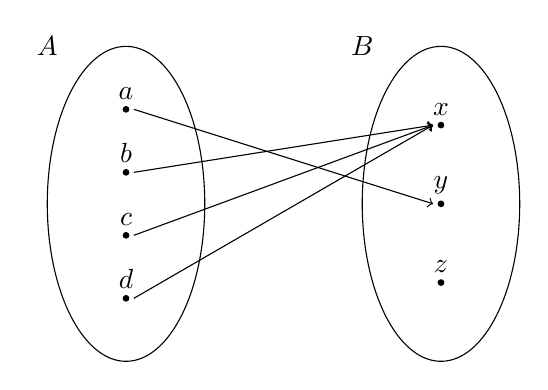
\begin{tikzpicture}
			\draw (0, 0) ellipse (1cm and 2cm);
			\draw (4, 0) ellipse (1cm and 2cm);
			\node at (-1, 2) {$A$};
			\node at (3, 2) {$B$};
			
			\draw[fill] (0, 1.2) circle (1pt) node[above]{$a$};
			\draw[fill] (0, 0.4) circle (1pt) node[above]{$b$};
			\draw[fill] (0, -0.4) circle (1pt) node[above]{$c$};
			\draw[fill] (0, -1.2) circle (1pt) node[above]{$d$};
			
			\draw[fill] (4, 1) circle (1pt) node[above]{$x$};
			\draw[fill] (4, 0) circle (1pt) node[above]{$y$};
			\draw[fill] (4, -1) circle (1pt) node[above]{$z$};
			
			\draw[->] (0.1, 1.2)--(3.9, 0);
			\draw[->] (0.1, 0.4)--(3.9, 1);
			\draw[->] (0.1, -0.4)--(3.9, 1);
			\draw[->] (0.1, -1.2)--(3.9, 1);
		\end{tikzpicture}
		\caption{Visual representation of the function $f:A\rightarrow B$.}
	\end{figure}
	
	\noindent As one may check, properties (F1) and (F2) hold, so $f$ is a function. 
\end{example}

\begin{example}\label{ch1ex_fn_set}
	Let $A = \{a, b, c, d\}$ and $B = \cc{P}(A)$ where $a, b, c, d$ are distinct elements. 
	Let $P$ be the predicate
	\[ P(t)\equiv \exists x\, (x\in A\land t = \langle x, \{x\}\rangle). \]
	By the existence of $A\times_{K} B$ and separation, we obtain the set $G_{f} = \{ t\in A\times_{K} B \,|\, P(t) \}$ and we form $f = \langle G_{f}, \langle A, B\rangle\rangle$. 
	As one may check, properties (F1) and (F2) hold, so $f$ is a function. 
\end{example}

Below we define some important sets that are associated with partial functions (which includes functions).

\begin{definition} 
	Let $f:A\rightharpoonup B$ be a partial function and let $S$ be its active domain.
	We define the \textbf{image} of $f$ to be 
	\[ \im f = \{ y\in B \;|\; y = f(x) \text{ for some } x\in S \}. \]
	If $E\subseteq A$, we define the \textbf{image of $E$ under $f$} to be
	\[ f(E) = \{ y\in B \;|\; y = f(x) \text{ for some } x\in E\cap S \}. \]
	If $F\subseteq B$, we define the \textbf{inverse image of $F$ under $f$} to be
	\[ f^{-1}(F) = \{ x\in S \;|\; f(x)\in F \}. \]
	Constructions justifying existence and uniqueness of these is done below. 
\end{definition}

For any partial function, let $\textrm{AmbDom}(f)$ be the ambient domain of $f$, let $\textrm{ActDom}(f)$ be the active domain of $f$, and let $\textrm{Cod}(f)$ be the codomain of $f$.
In the case where $f$ is a function, the active and ambient domains are the same and we just call them the domain $\textrm{Dom}(f)$. 
Define the predicate
\begin{align*}
	P(y, c) &\equiv (c\text{ is a Kuratowski ordered pair})\land (\pi_{L}(c)\text{ is a partial function}) \\
	&\quad\land \pi_{R}(c)\subseteq\textrm{AmbDom}(\pi_{L}(c))\land \exists x\, (x\in\pi_{R}(c)\cap\textrm{ActDom}(\pi_{L}(c))\land y = \textrm{App}(\pi_{L}(c), x)),
\end{align*}
and let $D(f, E)$ say $f$ is a partial function and $E\subseteq\textrm{AmbDom}(f)$. 
Then for all $f, E$ such that $D(f, E)$ holds, by separation there exists a unique set of the form
\[ \textrm{AppIm}(f, E) = \textrm{Sep}_{P}(\textrm{Cod}(f), \langle f, E\rangle), \]
where $\textrm{Sep}_{P}(A, c)$ is the subset of $A$ of elements $y$ satisfying $P(y, c)$, so $\textrm{AppIm}$ is defined for all $f, E$ for which $D(f, E)$ holds. 
Now $\textrm{AppIm}(f, E)$ is precisely the image of $E$ under $f$, and we abbreviate it as $f(E)$ as in the above definition. 
The image of $f$ is now simply $\im f = \textrm{AppIm}(f, \textrm{AmbDom}(f))$. 
The existence and uniqueness of inverse images can be shown similarly. 

\begin{example}
	Recall the function from \Cref{ch1ex_fn} where $A = \{a, b, c, d\}$, $B = \{x, y, z\}$, and $f:A\rightarrow B$ is defined by $f(a) = y$, $f(b) = x$, $f(c) = x$, and $f(d) = x$. 
	The codomain is $B = \{x, y, z\}$, but the image is $\im f = \{x, y\}$.
\end{example}

\begin{example}
	Recall the function from \Cref{ch1ex_fn_set} where $A = \{a, b, c, d\}$, $B = \cc{P}(A)$, and $f:A\rightarrow B$ is defined by $f(x) = \{x\}$. 
	The codomain is $\cc{P}(A)$, but the image is $\im f = \{\{a\}, \{b\}, \{c\}, \{d\}\}$.
\end{example}

Given two sets, we may consider all possible functions from one to the other.

\begin{definition}
	Given sets $A$ and $B$, the set of all functions $f:A\rightarrow B$ from $A$ to $B$ is denoted by $B^{A}$ or $\map(A, B)$.
\end{definition}

\noindent Let us justify the existence of $\map(A, B)$ given sets $A, B$. 

\begin{prop}
	Given sets $A$ and $B$, the set of all functions from $A$ to $B$ exists and is unique. 
\end{prop}
\begin{proof}
	First, we collect all graphs of functions from $A$ to $B$ into a set as follows. 
	By taking the power set, we obtain $\cc{P}(A\times _{K} B)$. 
	This is the collection of all sets $G\subseteq A\times_{K} B$.
	Let $P$ be the predicate
	\begin{align*}
		P(G, c) &\equiv (c\text{ is a Kuratowski ordered pair})\land G\subseteq\pi_{L}(c)\times_{K} \pi_{R}(c) \\
		&\quad\land (G\text{ satisfies (F1) and (F2) with respect to }\pi_{L}(c)\times_{K} \pi_{R}(c)).
	\end{align*}
	By separation, there exists a set
	\[ F = \{ G\in\cc{P}(A\times_{K} B) \,|\, P(G, \langle A, B\rangle) \}. \]
	This is the set of graphs of functions from $A$ to $B$. 
	
	To proceed, we invoke the axiom schema of replacement (ZFC7) to attach the domain and codomain to the graphs. 
	Let $Q$ be the predicate
	\begin{align*}
		Q(G, f, c) &\equiv f = \langle G, c\rangle.
	\end{align*}
	Let us check that this is a functional predicate. 
	Given $G$ and $c$, we may form $f = \langle G, c\rangle$.
	If $Q(G, f, c)$ and $Q(G, \wt{f}, c)$, then $f, \wt{f}$ are both $\langle G, c\rangle$, so $f = \wt{f}$. 
	Thus, $Q$ is a functional predicate and by the axiom schema of replacement (ZFC7) with parameter $c = \langle A, B\rangle$, there exists a set $\wt{F} = \textrm{Rep}_{Q}(F, \langle A, B\rangle)$ such that the following holds:
	
	\begin{enumerate}[itemsep=-0.4ex, label=(\roman*)]
		\item If $f\in\wt{F}$, then there exists $G\in F$ such that $Q(G, f, \langle A, B\rangle)$, so $f = \langle G, \langle A, B\rangle\rangle$.
		\item If $G\in F$, then there exists $f\in\wt{F}$ such that $Q(G, f, \langle A, B\rangle)$, so $f = \langle G, \langle A, B\rangle\rangle$. 
	\end{enumerate}
	
	\noindent So, given $A, B$, we took 
	\[ \wt{F} = \textrm{Rep}_{Q}(\textrm{Sep}_{P}(\cc{P}(A\times_{K} B), \langle A, B\rangle), \langle A, B\rangle). \]
	
	Next, we verify $\wt{F}$ is the set of all maps from $A$ to $B$ as intended.
	Suppose $f$ is a function from $A$ to $B$. 
	By definition, $f = \langle G_{f}, \langle A, B\rangle\rangle$ such that $G_{f}\subseteq A\times_{K} B$ satisfies (F1) and (F2). 
	We find $G_{f}\in F$, so by property (ii), there exists some $\wt{f}\in\wt{F}$ such that 
	\[ \wt{f} = \langle G_{f}, \langle A, B\rangle\rangle. \]
	The right-hand side is precisely $f$, so $f\in\wt{F}$. 
	Conversely, suppose $f\in\wt{F}$. 
	By property (i), there exists some $G\in F$ such that $f = \langle G, \langle A, B\rangle\rangle$.
	Given that $G\in F$, $G$ satisfies (F1) and (F2), so $f$ is a function.
	
	Thus, $f$ is a function from $A$ to $B$ if and only if $f\in\wt{F}$. 
	The uniqueness of the set of all functions from $A$ to $B$ follows straightforwardly by extensionality. 
\end{proof}

\subsection{Compositions and Changes of Domain and Codomain}

We will be using the following useful lemma.

\begin{lemma}\label{ch1thm_lemma_equality_of_fns}
	Suppose $f, g : A\rightarrow B$ are functions with the same domain $A$ and codomain $B$. 
	If $f(x) = g(x)$ for all $x\in A$, then $f = g$.
\end{lemma}
\begin{proof}
	Write $f = \langle G_{f}, \langle A, B\rangle\rangle$ and $g = \langle G_{g}, \langle A, B\rangle\rangle$. 
	We aim to show the graphs $G_{f}, G_{g}$ are equal. 
	Given $t\in G_{f}$, we know $t = \langle x, f(x)\rangle$ for some $x\in A$. 
	Since $f(x) = g(x)$ by hypothesis, substitution implies $t = \langle x, g(x)\rangle$, and $\langle x, g(x)\rangle\in G_{g}$. 
	Thus, by substitution, $t\in G_{g}$. 
	Conversely, if $t\in G_{g}$, analogous reasoning shows $t\in G_{f}$. 
	By extensionality, $G_{f} = G_{g}$ and so $f = g$. 
\end{proof}

We introduce composition of functions.

\begin{definition}[Composition]
	Let $f:A\rightarrow B$ and $g:B\rightarrow C$ be functions.
	We define the \textbf{composition} of these two functions to be the function $g\circ f:A\rightarrow C$ such that $g\circ f(a) = g(f(a))$ for all $a\in A$. 
	We verify $g\circ f$ exists and is unique below. 
\end{definition}

\begin{prop}[Existence and uniqueness of compositions]
	If $f:A\rightarrow B$ and $g:B\rightarrow C$ are functions, then the composition $g\circ f$ exists and is unique.
\end{prop}
\begin{proof}
	Write $f = \langle G_{f}, \langle A, B\rangle\rangle$ and $g = \langle G_{g}, \langle B, C\rangle\rangle$.
	By the existence of $A\times_{K} C$ and by separation, there exists the set
	\[ G = \{ t\in A\times_{K} C \,|\, t = \langle x, g(f(x))\rangle \text{ for some } x\in A \}. \]
	More formally, this is
	\[ G = \{ t\in A\times_{K} C \,|\, P(t, \langle f, g\rangle) \} \]
	where
	\begin{align*}
		P(t, c)&\equiv (c\text{ is a Kuratowski ordered pair})\land (\pi_{L}(c), \pi_{R}(c)\text{ are functions}) \\
		&\quad\land \textrm{Cod}(\pi_{L}(c)) = \textrm{Dom}(\pi_{R}(c)) \\
		&\quad\land \exists x\, (x\in\textrm{Dom}(\pi_{L}(c)) \land t = \langle x, \textrm{App}(\pi_{R}(c), \textrm{App}(\pi_{L}(c), x))\rangle).
	\end{align*}
	Now define $h = \langle G, \langle A, C\rangle\rangle$, which exists.
	Since $G\subseteq A\times_{K} C$, it remains to verify (F1) and (F2).
	
	For (F1), for each $x\in A$, we have $\langle x, g(f(x))\rangle\in A\times_{K} C$ and $P(\langle x, g(f(x))\rangle, \langle f, g\rangle)$, so 
	\[ \langle x, g(f(x))\rangle\in G, \] 
	so (F1) holds.
	For (F2), suppose $x\in A$ and $z, z'\in C$ such that 
	\[ \langle x, z\rangle, \langle x, z'\rangle\in G. \]
	By definition of $G$, there exist $u, u'\in A$ such that
	\[ \langle x, z\rangle = \langle u, g(f(u))\rangle \quad\text{and}\quad \langle x, z'\rangle = \langle u', g(f(u'))\rangle. \]
	By \Cref{ch1eqn_kuratowski_pair_property}, $x = u$, $z = g(f(u))$, $x = u'$, and $z' = g(f(u'))$.
	As a result we have $u = u'$, so by substitution, $g(f(u)) = g(f(u'))$, and so $z = z'$ and (F2) holds.
	
	This shows $h:A\rightarrow C$ is a function such that $h(x) = g(f(x))$ for all $x\in A$ by construction. 
	Uniqueness follows from \Cref{ch1thm_lemma_equality_of_fns}.
\end{proof}

By existence and uniqueness of $g\circ f$ given composable functions $f, g$, we may create a composition formation operator as follows.
Take the domain condition $D$ and predicate $P$ so that 
\[ D(f, g)\equiv (f, g\textrm{ are functions})\land \textrm{Cod}(f) = \textrm{Dom}(g) \] 
and 
\begin{align*}
	P(f, g, h)&\equiv D(f, g)\land (h\text{ is a function})\land \textrm{Dom}(h) = \textrm{Dom}(f) \\
	&\quad\land \textrm{Cod}(h) = \textrm{Cod}(g)\land \forall x\in\textrm{Dom}(f)\, (h(x) = g(f(x))). 
\end{align*}
Given 
\[ \forall f\forall g\, (D(f, g)\implies \exists ! h\, P(f, g, h)), \]
we obtain the operation $\textrm{Comp}$ with domain condition $D$ such that $h = \textrm{Comp}(f, g)$ is the composition. 
We abbreviate $\textrm{Comp}(f, g)$ as $g\circ f$. 

We introduce changes of domains and codomains of functions. 

\begin{definition}[Change of domain and codomain]
	Let $f:A\rightarrow B$, $X\subseteq A$, and $Y\supseteq f(X)$.
	We define $f|_{X}^{Y}$ to be the function from $X$ to $Y$ such that $f|_{X}^{Y}(x) = f(x)$ for all $x\in X$. 
	Notation for special cases:
	\begin{itemize}[itemsep=-0.4ex]
		\item If $Y = B$ (the codomain isn't changed), we write $f|_{X}^{B} = f|_{X}$.
		\item If $X = A$ (the domain isn't changed), we write $f|_{A}^{Y} = f|^{Y}$. 
	\end{itemize}
	\noindent We verify $f|_{X}^{Y}$ exists and is unique below. 
\end{definition}

\begin{prop}[Existence and uniqueness of change of domain and codomain]
	If $f:A\rightarrow B$ is a function, $X\subseteq A$, and $Y\supseteq f(X)$, then the function with a change of domain and codomain $f|_{X}^{Y}$ exists and is unique. 
\end{prop}
\begin{proof}
	Given $f = \langle G_{f}, \langle A, B\rangle\rangle$, $X\subseteq A$, and $Y\supseteq f(X)$, use separation to obtain the subset
	\[ G = \{ t\in G_{f} \,|\, t\in X\times_{K} Y \}. \]
	More formally, this is
	\[ G = \{ t\in G_{f} \,|\, P(t, \langle X, Y\rangle) \} \]
	where 
	\[ P(t, c)\equiv (c\text{ is a Kuratowski ordered pair})\land t\in \pi_{L}(c)\times_{K}\pi_{R}(c). \] 
	Now define $h = \langle G, \langle X, Y\rangle\rangle$, which exists. 
	If $t\in G$, then $P(t, \langle X, Y\rangle)$, so $t\in X\times_{K} Y$.
	Hence $G\subseteq X\times_{K} Y$, and it remains to verify (F1) and (F2). 
	
	For (F1), for each $x\in X$, we have $\langle x, f(x)\rangle\in G_{f}$ and $f(x)\in f(X)\subseteq Y$, and so $P(\langle x, f(x)\rangle, \langle X, Y\rangle)$. 
	Thus, 
	\[ \langle x, f(x)\rangle\in G, \] 
	so (F1) holds. 
	For (F2), suppose $x\in X$ and $y, y'\in Y$ such that 
	\[ \langle x, y\rangle, \langle x, y'\rangle \in G. \]
	Since $G\subseteq G_{f}$ and $G_{f}$ has property (F2), it follows $y = y'$, and so (F2) holds. 
	
	This shows $h:X\rightarrow Y$ is a function such that $h(x) = f(x)$ for all $x\in X$ by construction. 
	Uniqueness follows from \Cref{ch1thm_lemma_equality_of_fns}.
\end{proof}

By existence and uniqueness of $f|_{X}^{Y}$ given $f:A\rightarrow B$, $X\subseteq A$, and $Y\supseteq f(X)$, we may create a domain/codomain change operator as follows.
Take the domain condition $D$ and predicate $P$ so that
\begin{align*}
	D(f, p)&\equiv (f\text{ is a function})\land (p\text{ is a Kuratowski ordered pair}) \\
	&\quad\land \pi_{L}(p)\subseteq\textrm{Dom}(f)\land \pi_{R}(p)\supseteq f(\pi_{L}(p))
\end{align*}
and
\begin{align*}
	P(f, p, h)&\equiv D(f, p)\land (h\text{ is a function})\land \textrm{Dom}(h) = \pi_{L}(p) \\
	&\quad\land \textrm{Cod}(h) = \pi_{R}(p) \land \forall x\in\pi_{L}(p)\, (f(x) = h(x)). 
\end{align*}
Given
\[ \forall f\forall p\, (D(f, p)\implies \exists ! h\, P(f, p, h)), \]
we obtain the operation $\textrm{Change}$ with domain condition $D$ such that $h = \textrm{Change}(f, p)$ is the function obtained from $f$ by restricting the domain to $X = \pi_{L}(p)$ and changing the codomain to $Y = \pi_{R}(p)$. 
We abbreviate $\textrm{Change}(f, \langle X, Y\rangle)$ as $f|_{X}^{Y}$. 

\subsection{Identity Maps and Inverses}

Now we present some ubiquitous types of functions. 

\begin{definition}[The identity map]
	Given a set $A$, we define the \textbf{identity map} of $A$ to be the function denoted $\id_{A}:A\rightarrow A$ that outputs exactly the same element that is given as the input: $\id_{A}(x) = x$ for all $x\in A$. 
\end{definition}

\noindent We leave it to the reader to construct the identity map and prove uniqueness in the ending problem set. 

\begin{definition}
	Let $f:A\rightarrow B$ and $g:B\rightarrow A$ be maps.
	\begin{itemize}[itemsep=-0.4ex]
		\item $g$ is said to be a \textbf{left-inverse} of $f$ if $g\circ f = \id_{A}$.
		\item $g$ is said to be a \textbf{right-inverse} of $f$ if $f\circ g = \id_{B}$.
		\item $g$ is said to be an \textbf{inverse} of $f$ if it is both a left-inverse and right-inverse.
		We leave it to the reader to show that if it exists, then it is unique.
		We denote it by $f^{-1}$, which can be done due to uniqueness. 
	\end{itemize}
\end{definition}

\begin{example}[Left-inverse]
	Let $A = \{a, b, c\}$ and $B = \{x, y, z, w\}$ where $a, b, c, x, y, z, w$ are distinct elements. 
	Define $f:A\rightarrow B$ by $f(a) = x$, $f(b) = y$, and $f(c) = z$.
	Define $g:B\rightarrow A$ by $g(x) = a$, $g(y) = b$, $g(z) = c$, and $g(w) = c$.
	Then
	\[ g(f(a)) = a,\quad g(f(b)) = b,\quad\text{and}\quad g(f(c)) = c, \]
	so $g\circ f = \id_A$ and $g$ is a left-inverse of $f$.
	However, $f(g(w)) = z\ne w$, so $g$ is not a right-inverse of $f$.
\end{example}

\begin{example}[Right-inverse]
	Let $A = \{a, b, c, d\}$ and $B = \{x, y, z\}$ where $a, b, c, d, x, y, z$ are distinct elements. 
	Define $f:A\rightarrow B$ by $f(a) = x$, $f(b) = y$, $f(c) = z$, and $f(d) = z$.
	Define $g:B\rightarrow A$ by $g(x) = a$, $g(y) = b$, and $g(z) = c$.
	Then
	\[ f(g(x)) = x,\quad f(g(y)) = y,\quad\text{and}\quad f(g(z)) = z, \]
	so $f\circ g = \id_B$ and $g$ is a right-inverse of $f$.
	However, $g(f(d)) = c\ne d$, so $g$ is not a left-inverse of $f$.
\end{example}

\begin{example}[Inverse]
	Let $A = \{a, b, c\}$ and $B = \{x, y, z\}$ where $a, b, c, x, y, z$ are distinct elements.
	Define $f:A\rightarrow B$ by $f(a) = y$, $f(b) = z$, and $f(c) = x$.
	Define $g:B\rightarrow A$ by $g(x) = c$, $g(y) = a$, and $g(z) = b$.
	Then
	\[ g(f(a)) = a,\quad g(f(b)) = b,\quad\text{and}\quad g(f(c)) = c, \]
	so $g\circ f = \id_A$. 
	Also,
	\[ f(g(x)) = x,\quad f(g(y)) = y,\quad\text{and}\quad f(g(z)) = z, \]
	so $f\circ g = \id_B$.
	Thus, $g$ is an inverse of $f$.
\end{example}

\subsection{Injective, Surjective, and Bijective Maps}

\begin{definition}
	Let $f:A\rightarrow B$ be a function.
	\begin{itemize}[itemsep=-0.4ex]
		\item We say $f$ is \textbf{injective} if for all $x, y\in A$ we have $f(x) = f(y)\implies x = y$.
		\item We say $f$ is \textbf{surjective} if for all $y\in B$ there exists $x\in A$ such that $f(x) = y$.
		\item We say $f$ is \textbf{bijective} if it is both injective and surjective. 
	\end{itemize}
\end{definition}

An equivalent characterization of injective functions is that $f:A\rightarrow B$ is injective if and only if for all $x, y\in A$ such that $x\ne y$ we have $f(x) \ne f(y)$.
That is, injective functions send distinct elements to distinct elements. 
An equivalent characterization of surjective functions is that $f:A\rightarrow B$ is surjective if and only if $\im f = B$. 
That is, surjective functions are precisely the ones in which their image matches their codomain. 
We provide some illustrations of some examples below. 

\begin{figure}[H]
	\centering
	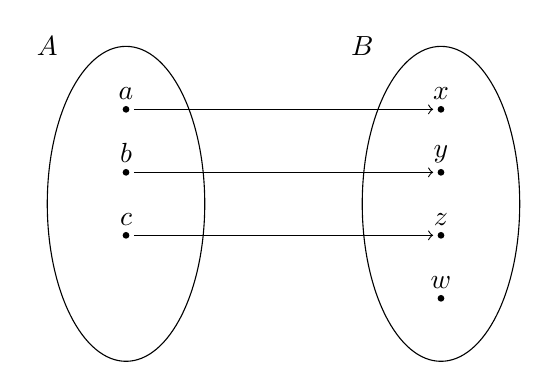
\begin{tikzpicture}
		\draw (0, 0) ellipse (1cm and 2cm);
		\draw (4, 0) ellipse (1cm and 2cm);
		\node at (-1, 2) {$A$};
		\node at (3, 2) {$B$};
		
		\draw[fill] (0, 1.2) circle (1pt) node[above]{$a$};
		\draw[fill] (0, 0.4) circle (1pt) node[above]{$b$};
		\draw[fill] (0, -0.4) circle (1pt) node[above]{$c$};
		
		\draw[fill] (4, 1.2) circle (1pt) node[above]{$x$};
		\draw[fill] (4, 0.4) circle (1pt) node[above]{$y$};
		\draw[fill] (4, -0.4) circle (1pt) node[above]{$z$};
		\draw[fill] (4, -1.2) circle (1pt) node[above]{$w$};
		
		\draw[->] (0.1, 1.2)--(3.9, 1.2);
		\draw[->] (0.1, 0.4)--(3.9, 0.4);
		\draw[->] (0.1, -0.4)--(3.9, -0.4);
	\end{tikzpicture}
	\caption{An injective but not surjective function.}
\end{figure}

\begin{figure}[H]
	\centering
	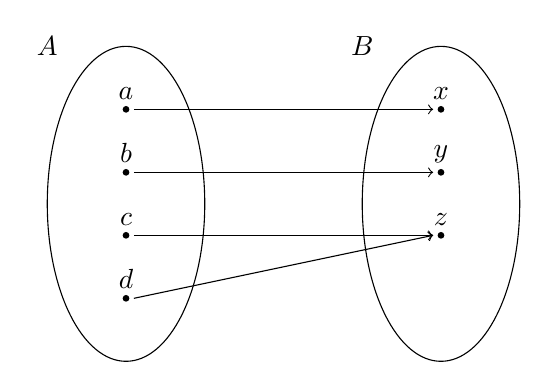
\begin{tikzpicture}
		\draw (0, 0) ellipse (1cm and 2cm);
		\draw (4, 0) ellipse (1cm and 2cm);
		\node at (-1, 2) {$A$};
		\node at (3, 2) {$B$};
		
		\draw[fill] (0, 1.2) circle (1pt) node[above]{$a$};
		\draw[fill] (0, 0.4) circle (1pt) node[above]{$b$};
		\draw[fill] (0, -0.4) circle (1pt) node[above]{$c$};
		\draw[fill] (0, -1.2) circle (1pt) node[above]{$d$};
		
		\draw[fill] (4, 1.2) circle (1pt) node[above]{$x$};
		\draw[fill] (4, 0.4) circle (1pt) node[above]{$y$};
		\draw[fill] (4, -0.4) circle (1pt) node[above]{$z$};
		
		\draw[->] (0.1, 1.2)--(3.9, 1.2);
		\draw[->] (0.1, 0.4)--(3.9, 0.4);
		\draw[->] (0.1, -0.4)--(3.9, -0.4);
		\draw[->] (0.1, -1.2)--(3.9, -0.4);
	\end{tikzpicture}
	\caption{A surjective but not injective function.}
\end{figure}

\begin{figure}[htbp]
	\centering
	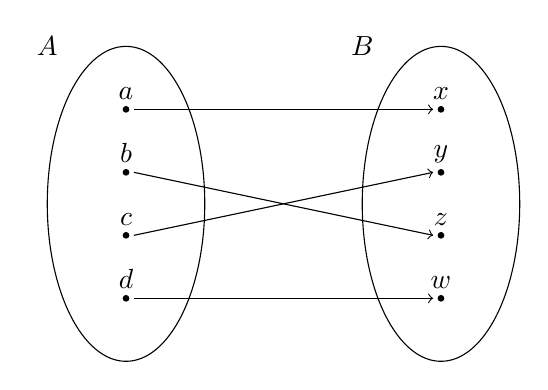
\begin{tikzpicture}
		\draw (0, 0) ellipse (1cm and 2cm);
		\draw (4, 0) ellipse (1cm and 2cm);
		\node at (-1, 2) {$A$};
		\node at (3, 2) {$B$};
		
		\draw[fill] (0, 1.2) circle (1pt) node[above]{$a$};
		\draw[fill] (0, 0.4) circle (1pt) node[above]{$b$};
		\draw[fill] (0, -0.4) circle (1pt) node[above]{$c$};
		\draw[fill] (0, -1.2) circle (1pt) node[above]{$d$};
		
		\draw[fill] (4, 1.2) circle (1pt) node[above]{$x$};
		\draw[fill] (4, 0.4) circle (1pt) node[above]{$y$};
		\draw[fill] (4, -0.4) circle (1pt) node[above]{$z$};
		\draw[fill] (4, -1.2) circle (1pt) node[above]{$w$};
		
		\draw[->] (0.1, 1.2)--(3.9, 1.2);
		\draw[->] (0.1, 0.4)--(3.9, -0.4);
		\draw[->] (0.1, -0.4)--(3.9, 0.4);
		\draw[->] (0.1, -1.2)--(3.9, -1.2);
	\end{tikzpicture}
	\caption{A bijective function.}
\end{figure}

\begin{figure}[H]
	\centering
	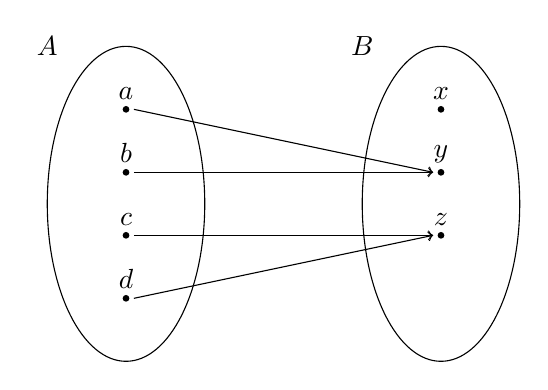
\begin{tikzpicture}
		\draw (0, 0) ellipse (1cm and 2cm);
		\draw (4, 0) ellipse (1cm and 2cm);
		\node at (-1, 2) {$A$};
		\node at (3, 2) {$B$};
		
		\draw[fill] (0, 1.2) circle (1pt) node[above]{$a$};
		\draw[fill] (0, 0.4) circle (1pt) node[above]{$b$};
		\draw[fill] (0, -0.4) circle (1pt) node[above]{$c$};
		\draw[fill] (0, -1.2) circle (1pt) node[above]{$d$};
		
		\draw[fill] (4, 1.2) circle (1pt) node[above]{$x$};
		\draw[fill] (4, 0.4) circle (1pt) node[above]{$y$};
		\draw[fill] (4, -0.4) circle (1pt) node[above]{$z$};
		
		\draw[->] (0.1, 1.2)--(3.9, 0.4);
		\draw[->] (0.1, 0.4)--(3.9, 0.4);
		\draw[->] (0.1, -0.4)--(3.9, -0.4);
		\draw[->] (0.1, -1.2)--(3.9, -0.4);
	\end{tikzpicture}
	\caption{A function that is neither injective nor surjective.}
\end{figure}

\subsection{Functions and Quotients}

Let us revisit the notion of equivalence classes and quotient sets. 
Given a set $A$ and an equivalence relation $\sim$ on $A$, the quotient set $A/\sim$ is defined as
\[ A/\sim\; = \{ x\in\cc{P}(A) \,|\, x = [a] \text{ for some } a\in A \} \quad\text{where}\quad [a] = \{ a'\in A \,|\, a\sim a' \} \]
for each $a\in A$. 
We often want to define functions on quotient sets, which would be of the form $f:A/\sim\;\rightarrow B$. 
However, we have to be careful:
If we define $f([a])$ in terms of a representative $a$ of the equivalence class $[a]$, we must ensure that the resulting value is independent of the choice of representative.
If $a\sim a'$, then the rule used to define $f([a])$ must assign the same value whether we started with representative $a$ or representative $a'$.
If this does not hold, then in informal treatments we say the function is \textbf{not well-defined}. 
Formally speaking, this actually means the function simply does not exist. 

\begin{example}[$f$ is not well-defined]\label{ch1ex_f_not_well_defd}
	Let $A = \{a, i, b, j, c, k\}$ and $B = \{x, y\}$ where all elements listed are distinct from one another.
	Let $P(t)\equiv t = i\lor t = j\lor t = k$.
	Define a relation $\sim$ on $A$ by
	\begin{align*}
		a\sim a, \qquad i\sim i, \qquad b\sim b, \qquad j\sim j, \qquad c\sim c, \qquad k\sim k, \\
		a\sim i, \qquad i\sim a, \qquad b\sim j, \qquad j\sim b, \qquad c\sim k, \qquad k\sim c.
	\end{align*}
	We leave it to the reader to check this is an equivalence relation on $A$.
	The resulting quotient set is 
	\[ A/\sim\; = \{\{a, i\}, \{b, j\}, \{c, k\}\}. \]
	Define $f:A/\sim\;\rightarrow B$ as follows:
	\begin{align*}
		f([\alpha]) = \begin{cases}
			x &\text{ if } P(\alpha), \\
			y &\text{ otherwise}.
		\end{cases}
	\end{align*}
	This function is not well-defined!
	The problem is that because $[a] = [i]$, it must be the case that $f([a]) = f([i])$, but if we follow our naive rule then $f([a]) = x$ and $f([i]) = y$.
	
	On one hand, $f([a]) = f([i])$ but we declared at the start that $x$ and $y$ are distinct elements: $x\ne y$. 
	The mere introduction of this function drives us into a contradiction, so it must not exist. 
	This is where it is necessary to fall back to set-theoretic constructions as in \Cref{ch1ex_fn} and \Cref{ch1ex_fn_set}. 
\end{example}

Below, we provide the appropriate definitions and theorems needed to describe a fool-proof recipe for defining functions on quotient sets. 

\begin{definition}
	If $\sim$ is an equivalence relation on a set $A$, the map $q:A\rightarrow A/\sim$ defined by $q(a) = [a]$ is called the \textbf{quotient map}. 
\end{definition}

Here is our construction for the above definition. 
Given any relation $R = \langle G_{R}, \langle A, B\rangle\rangle$, we take $\textrm{Dom}(R) = A$ and $\textrm{Cod}(R) = B$. 
Take $A\times_{K} A/\sim$ and apply separation to get
\[ G_{q} = \{ t\in A\times_{K} A/\sim \,|\, P(t, \sim) \} \]
where
\[ P(t, \sim)\equiv (\sim\text{ is an equivalence relation})\land \exists a\in\textrm{Dom}(c)\, (t = \langle a, \textrm{EquivCl}(a, \sim)\rangle) \]
where if $\sim$ is an equivalence relation on $A = \textrm{Dom}(\sim)$ and $a\in A$ then $\textrm{EquivCl}(a, \sim)$ is the equivalence class $[a]\in A/\sim$. 
Here $G_{q}\subseteq A\times_{K} A/\sim$ and the reader may verify that it satisfies (F1) and (F2). 
By forming $q = \langle G_{q}, \langle A, A/\sim\rangle\rangle$, we verify that $q$ indeed exists as a function. 

\begin{lemma}
	If $\sim$ is an equivalence relation on a set $A$, then the quotient map $q:A\rightarrow A/\sim$ is surjective.
\end{lemma}
\begin{proof}
	If $x\in A/\sim$ then $x = [a]$ for some $a\in A$, so $q(a) = x$. 
\end{proof}

Now we describe the main strategy for defining functions on quotient sets. 
Given a set $A$ with an equivalence relation $\sim$, instead of trying to define a map $g:A/\sim\;\rightarrow B$ directly on domain $A/\sim$ (which may result in an inconsistent definition like in \Cref{ch1ex_f_not_well_defd} if we are not careful), it makes sense to define a map $f:A\rightarrow B$ on domain $A$, and if this map $f$ meets certain conditions, it passes to a corresponding map $g:A/\sim\;\rightarrow B$ guaranteed to be well-defined. 
This is justified and made precise by the theorem below. 

\begin{theorem}[Quotient factorization theorem for sets]\label{ch1thm_quotient_factor_thm}
	Suppose $\sim$ is an equivalence relation on a set $A$ and $f:A\rightarrow B$ is a function such that $a\sim a'$ implies $f(a) = f(a')$ for all $a, a'\in A$. 
	Then there exists a unique function $g:A/\sim\;\rightarrow B$ such that 
	\begin{align}\label{ch1eqn_quotient_factor_comm}
		f = g\circ q
	\end{align}
	where $q$ is the quotient map with respect to $\sim$. 
\end{theorem}
\begin{figure}[H]
	\centering
	\begin{tikzpicture}[node distance=2.8cm and 3.5cm, auto]
		\node (A) at (0 ,0) {$A$};
		\node (B) at (0, -2.5) {$A/\sim$};
		\node (C) at (2.5, 0) {$B$};
		
		\draw[->] (A) to node[left] {$q$} (B);
		\draw[->] (A) to node[above] {$f$} (C);
		\draw[->, dashed] (B) to node[below right] {$g$} (C);
	\end{tikzpicture}
	\caption{A commutative diagram illustrating the quotient factorization theorem for sets.
	A \textbf{commutative diagram} is a diagram of objects and functions in which any two paths with the same start and end points yield the same output for each input.}
\end{figure}
\begin{proof}
	\textsc{Existence.}
	Let $Q = A/\!\sim$, let $q:A\rightarrow Q$ be the quotient map, and form the product $Q\times_{K} B$.
	By separation, take the set
	\[ G_{g} = \{ t\in Q\times_{K} B \,|\, t = \langle [a], f(a)\rangle \text{ for some } a\in A \}. \]
	Formally, this is
	\[ G_{g} = \{ t\in Q\times_{K} B \,|\, P(t, \langle f, \sim\rangle) \} \]
	where 
	\begin{align*}
		P(t, c)&\equiv (c\text{ is a Kuratowski ordered pair})\land (\pi_{L}(c)\text{ is a function}) \\
		&\quad\land (\pi_{R}(c)\text{ is an equivalence relation}) \\
		&\quad\land \exists a\in\textrm{Dom}(\pi_{L}(c))\, (t = \langle \textrm{EquivCl}(a, \pi_{R}(c)), \textrm{App}(\pi_{L}(c), a)\rangle ). 
	\end{align*}
	Now form $g = \langle G_{g}, \langle Q, B\rangle\rangle$, which exists. 
	If $t\in G_{g}$, then $t = \langle [a], f(a)\rangle$ for some $a\in A$, so $t\in Q\times_{K} B$.
	Thus, $G_{g}\subseteq Q\times_{K}B$, and it remains to show it satisfies (F1) and (F2). 
	
	For (F1), let $x\in Q$.
	By definition of quotients, there exists $a\in A$ such that $x = [a]$. 
	Given that $f(a)\in B$, 
	\[ \langle x, f(a)\rangle = \langle [a], f(a)\rangle \in Q\times_{K} B, \]
	and also $P(\langle x, f(a)\rangle, \langle f, \sim\rangle)$ holds, so $\langle x, f(a)\rangle\in G_{g}$. 
	Thus, (F1) holds. 
	
	For (F2), suppose $x\in Q$ and $y, y'\in B$ such that
	\[ \langle x, y\rangle, \langle x, y'\rangle\in G_{g}. \]
	By definition of $G_{g}$, there exist $a, a;\in A$ such that
	\[ \langle x, y\rangle = \langle [a], f(a)\rangle \quad\text{and}\quad \langle x, y'\rangle = \langle [a'], f(a')\rangle. \]
	By \Cref{ch1eqn_kuratowski_pair_property}, 
	\[ x = [a], \quad y = f(a), \quad x = [a'], \quad\text{and}\quad y' = f(a'). \]
	So $[a] = [a']$, which implies $a\sim a'$ by \Cref{ch1eqn_equiv_classes_property}.
	By hypothesis of $f$, it follows $f(a) = f(a')$ and so $y = y'$. 
	Thus, (F2) holds. 
	This proves $g:Q\rightarrow B$ exists and is a function. 
	
	By construction, $g\circ q(a) = g(q(a)) = g([a]) = f(a)$ for all $a\in A$, so by \Cref{ch1thm_lemma_equality_of_fns},  \Cref{ch1eqn_quotient_factor_comm} holds. \\
	
	\textsc{Uniqueness.}
	Suppose $g, g': Q \rightarrow B$ are two functions such that $f = g\circ q$ and $f = g'\circ q$. 
	By hypothesis, $g$ and $g'$ have the same domain $Q$ and codomain $B$. 
	Given $x\in Q$, by construction of $Q$ we know $x = [a]$ for some $a\in A$.
	Then 
	\[ g(x) = g([a]) = g(q(a)) = f(a) = g'(q(a)) = g'([a]) = g'(x). \]
	This applies to all $x\in Q$, so by \Cref{ch1thm_lemma_equality_of_fns}, it follows $g = g'$. 
\end{proof}

\begin{example}
	Let $A = \{a, b, c, \rho, \sigma\}$ and $B = \{\textrm{Latin}, \textrm{Greek}\}$ where all elements listed are distinct. 
	Let $P(t)\equiv t = a\lor t = b\lor t = c$. 
	Define a relation $\sim$ on $A$ by
	\begin{align*}
		& a\sim a, \quad b\sim b, \quad c\sim c, \quad a\sim b, \quad b\sim a, \quad a\sim c, \quad c\sim a, \quad b\sim c, \quad c\sim b, \\
		& \rho\sim\rho, \quad \sigma\sim\sigma, \quad \rho\sim \sigma, \quad \sigma\sim \rho.
	\end{align*}
	We leave it to the reader to check this is an equivalence relation on $A$.
	The resulting quotient is 
	\[ A/\sim\; = \{\{a, b, c\}, \{\sigma, \rho\}\}. \]
	Instead of defining a function from $A/\sim$ to $B$ directly like we tried in \Cref{ch1ex_f_not_well_defd}, we follow the more principled approach by defining $f:A\rightarrow B$ by
	\[ f(x) = \begin{cases}
		\textrm{Latin} &\text{ if } P(x), \\
		\textrm{Greek} &\text{ otherwise}.
	\end{cases} \]
	Let us construct this function to ensure it exists. 
	Apply separation to $A\times_{K} B$ to obtain
	\[ G_{f} = \{ t\in A\times_{K} B \,|\, t = \langle x, \textrm{Latin}\rangle \text{ if } P(x) \text{ and } t = \langle x, \textrm{Greek}\rangle \text{ otherwise} \}. \]
	More formally, this is
	\[ G_{f} = \{ t\in A\times_{K} B \,|\, Q(t) \} \]
	where
	\[ Q(t)\equiv \exists x\, ((P(x)\implies t = \langle x, \textrm{Latin}\rangle)\land (\neg P(x)\implies t = \langle x, \textrm{Greek}\rangle)). \]
	We form $f = \langle G_{f}, \langle A, B\rangle\rangle$ and leave the reader to verify that $G_{f}\subseteq A\times_{K} B$, (F1), and (F2) hold, proving $f$ exists and is a function. 
	
	Now because 
	\[ f(a) = f(b) = f(c) = \textrm{Latin} \quad\text{and}\quad f(\rho) = f(\sigma) = \textrm{Greek}, \] 
	we have $x\sim x'$ implies $f(x) = f(x')$ for all $x, x'\in A$, and so \Cref{ch1thm_quotient_factor_thm} is applicable. 
	This, there exists a unique function $g:A/\sim\;\rightarrow B$ such that $f = g\circ q$ where $q$ is the quotient map. 
	In this case, 
	\[ g(\{a, b, c\}) = \textrm{Latin} \quad\text{and}\quad g(\{\rho, \sigma\}) = \textrm{Greek}. \]
	In more loose terms, we may say $g([x]) = \textrm{Latin}$ if $P(x)$ and $g([x]) = \textrm{Greek}$ if $\neg P(x)$ without running into trouble, because \Cref{ch1thm_quotient_factor_thm} guarantees this leaves $g$ as a well-defined map. 
\end{example}

\section{Choice and Extensionality Principles}

\subsection{The Axiom of Choice}


% \subsection{Zorn's Lemma}

% At the end, we will write the following topics
% 1. Peano system
% 2. Axiom of infinity
% 3. Principle of induction
% 4. Defining a total order on N
% Principle of recursive definitions
% Defining set operations
% Counting, Finite, and Infinite Sets
% Defining Addition and Multiplication
% Relative Cardinality
% Numerical Representations

% We intended to place everything on ZFC set theory.
% However, discussions of numeral representations of natraul numbers
% requires us to talk about written strings and characters, which are
% not sets (Godel encodings or sequences don't count). 

% The intention is to consider placing everything on 2-level homotopy type theory
% so that both the theory and metatheory are subsumed by one framework. 
% It may still be possible to define the numeral system in first-order logic + 
% ZFC set theory, but I am not sure how satisfying it would be. 

\iffalse 
\subsection{The Axiom of Choice}

We introduce the following axiom.

\begin{enumerate}[itemsep=-0.4ex, label=\textup{(ZFC${\arabic*}$)}]\setcounter{enumi}{8}
	\item\textsc{Axiom of Choice.}
	Given a set $A$ consisting of nonempty sets, there exists a function
	\[ f:A\rightarrow\bigcup A \]
	such that $f(a)\in a$ for all $a\in A$. 
\end{enumerate}

Any function matching the description of $f$ in (ZFC9) is called a \textbf{choice function}.
The meaning of such a function is that for each $a\in A$, the function picks out some specific element of $a$. 

\begin{exer}\label{ch1thm_fn_inverses}
	Let $f:A\rightarrow B$ be a map whose domain $A$ is nonempty. 
	Prove the following statements:
	\begin{itemize}[itemsep=-0.4ex]
		\item $f$ is injective if and only if it has a left-inverse.
		If the left-inverse exists, it is surjective.
		\item $f$ is surjective if and only if it has a right-inverse.
		If the right-inverse exists, it is injective.
		\item $f$ is bijective if and only if it has an inverse.
		If the inverse exists, it is bijective. 
	\end{itemize}
	The second bullet point requires the use of the axiom of choice. 
\end{exer}

A famous consequence of the axiom of choice is Zorn's lemma.
Zorn's lemma is in fact equivalent to the axiom of choice (given all the other axioms), but for the purposes of our text we are concerned with only one implication direction. 

\begin{theorem}[Zorn's lemma]\label{ch1thm_zornslemma}
	Let $(P, <)$ be a nonempty partially ordered set.
	If every totally ordered subset $C\subseteq P$ \textup{(}whose order relation is passed down from $P$\textup{)} is bounded above, then there exists a maximal element of $P$.
\end{theorem}

The proof for Zorn's lemma is long and difficult, so we place it in \Cref{chA_set_theory_pfs}. 




\section{The Peano System and The Axiom of Infinity}

\subsection{The Peano System}

The natural numbers are indispensable objects of mathematics. 
At the most basic level, they are used to count things, and in set theory, we need a way to keep track of how many elements there are in a set.
Before we can study the natural numbers as a fully developed number system with arithmetic, we will first isolate their fundamental properties in a simpler form. 

\begin{definition}
	A \textbf{Peano system} is a set $\bb{N}$ with a distinguished object $0\in\bb{N}$ and a function $\sigma:\bb{N}\rightarrow\bb{N}$, called a \textbf{successor operator}, such that the following axioms hold:
	\begin{enumerate}[itemsep=-0.0ex, label=\textup{(\textup{PA}\arabic*)}]
		\item There is no element $b\in \bb{N}$ such that $\sigma(b) = 0$.
		\item $\sigma$ is injective.
		\item\textsc{(Induction).} 
		If $A$ is a subset of $\bb{N}$ such that $0\in A$ and $a\in A\implies \sigma(a)\in A$, then $A = \bb{N}$. 
	\end{enumerate}
	We refer to elements of $\bb{N}$ as \textbf{natural numbers}.
	We may denote a Peano system as $(\bb{N}, 0, \sigma)$ to emphasize that the set $\bb{N}$ comes with a special element $0$ and a function $\sigma$. 
	Often, however, we will simply refer to it by its set $\bb{N}$, leaving $0$ and $\sigma$ implicit. 
\end{definition}

Axioms (PA1)--(PA3) are a condensed reformulation of the \textbf{Peano axioms}.
Traditionally, they are presented as a list of five axioms, but the exact number varies depending on how one formulates them.
Giuseppe Peano (1858--1932) originally presented them as a list of nine axioms. 
So far we have defined a Peano system, but we have not shown that such a structure actually exists within our set-theoretic framework. 
To do this within set theory, we require one more axiom.



\subsection{The Axiom of Infinity}

We introduce the final axiom of ZFC with which we are able to provide an example of a Peano system from within set theory. 

\begin{enumerate}[itemsep=-0.4ex, label=\textup{(ZFC${\arabic*}$)}]\setcounter{enumi}{9}
	\item\textsc{Axiom of Infinity.}
	There exists a set $I$ for which the following holds: $\varnothing\in I$, and for all objects $x$, if $x\in I$ then $x\cup\{x\}\in I$. 
\end{enumerate}

Given a set $A$, define the \textbf{von Neumann successor} of $A$ to be the set $S(A) = A\cup\{A\}$. 
If $I$ is a set for which $\varnothing\in I$, and $S(A)\in I$ for every $A\in I$, we say $I$ is an \textbf{inductive set}.
Thus, (ZFC10) asserts the existence of an inductive set. 
Now if $I$ is an inductive set, define
\[ \omega_{I} = \bigcap \{ J\subseteq I \;|\; J\text{ is an inductive set} \}. \]
Such a set exists by the axiom of power set (ZFC6), axiom schema of separation (ZFC5), and the existence of intersections. 

\begin{prop}\label{ch1thm_intersection_inductive}
	The intersection of any nonempty collection of inductive sets is an inductive set.
	Hence, if $I$ is an inductive set, then $\omega_{I}$ is an inductive set.
\end{prop}
\begin{proof}
	Let $\cc{A}$ be a nonempty collection of inductive sets, and let $K = \bigcap\cc{A}$.
	For every $I\in\cc{A}$, we have $\varnothing\in I$, so $\varnothing\in K$.
	If $A\in K$, then $A\in I$ for all $I\in\cc{A}$.
	Now if $A\in I$ and $I$ is inductive, then $S(A)\in I$, so it follows that $S(A)\in I$ for all $I\in\cc{A}$.
	Therefore, $S(A)\in K$.
	This shows $K$ is inductive.
\end{proof}

\begin{prop}\label{ch1thm_inductive_unique}
	If $I, J$ are inductive sets, then $\omega_{I} = \omega_{J}$.
\end{prop}
\begin{proof}
	By \Cref{ch1thm_intersection_inductive}, $\omega_{I}\cap J$ is an inductive subset of $J$, so then $\omega_{J}\subseteq\omega_{I}\cap J\subseteq\omega_{I}$.
	By the same reasoning but reversing the roles of $I$ and $J$, we find $\omega_{I}\subseteq I\cap\omega_{J}\subseteq\omega_{J}$.
	Thus $\omega_{I} = \omega_{J}$.
\end{proof}

We define $\omega = \omega_{I}$ where $I$ is any inductive set.
By \Cref{ch1thm_inductive_unique}, this set does not depend on the choice of $I$. 
To get a sense of what $\omega$ looks like, we label the following elements:
\begin{alignat*}{2}
	0 &= \varnothing &&= \varnothing, \\
	1 &= 0 \cup \{0\} &&= \{0\}, \\
	2 &= 1 \cup \{1\} &&= \{0, 1\}, \\
	3 &= 2 \cup \{2\} &&= \{0, 1, 2\}, \\
	4 &= 3 \cup \{3\} &&= \{0, 1, 2, 3\}.
\end{alignat*}
No matter how far we continue this pattern, we will not be able to exhaust the set. 
In other words, the pattern is endless. 
This is called the \textbf{von Neumann construction of the natural numbers}, named after John von Neumann (1903--1957).
Let us show that $\omega$ has precisely the structure of a Peano system.

\begin{prop}\label{ch1thm_nat_satisfy_Peano}
	There exists an element $0\in\omega$ and a function $\sigma:\omega\rightarrow\omega$ such that the Peano axioms are satisfied.
\end{prop}
\begin{proof}
	Define $0 = \varnothing$ and $\sigma:\omega\rightarrow\omega$ by $\sigma(a) = S(a)$. 
	We leave it to the reader to verify $\sigma = ((\omega, \omega)_{K}, G_{\sigma})_{K}$ exists.
	We will show these satisfy (PA1)--(PA3) from the definition of Peano systems. 
	
	(PA1).
	For any $b\in\omega$, we have $\sigma(b) = b\cup\{b\}$, so $b\in\sigma(b)$ which implies $\sigma(b)\ne\varnothing = 0$.
	
	(PA2).
	Suppose $\sigma(a) = \sigma(b)$ for any distinct $a, b\in\omega$. 
	The inequality $a\ne b$ and the fact that $a\cup\{a\} = b\cup\{b\}$ together imply $a\in b$ and $b\in a$. 
	This runs into conflict with the axioms of pairing (ZFC3) and foundation (ZFC8):
	By pairing, we may form the set $\{a, b\}$.
	By foundation, there exists $x\in\{a, b\}$ such that $x\cap\{a, b\} = \varnothing$.
	Now $x\in\{a, b\}$ implies $x=a$ or $x=b$. 
	In the former case, $a\cap \{a, b\} = \varnothing$, but $b\in a$ and $b\in\{a, b\}$, so $b\in a\cap \{a, b\}$, which is a contradiction.
	In the latter case, we obtain an analogous contradiction. 
	Thus, if $\sigma(a) = \sigma(b)$ then $a=b$. 
	This proves $\sigma$ is injective.
	
	(PA3).
	Suppose $A\subseteq\omega$, $0\in A$, and $a\in A\implies\sigma(a)\in A$.
	Then $A$ is an inductive set, so $A\subseteq\omega = \omega_{A}\subseteq A$ (remember $\omega = \omega_{I}$ for any inductive set $I$). 
	Given $A\subseteq\omega$ and $\omega\subseteq A$, we conclude $A = \omega$, as desired. 
\end{proof}

What we have done is show that $(\omega, 0, \sigma)$ is an instantiation of a Peano system $(\bb{N}, 0, \sigma)$. 
In this chapter, we only need to know that at least one such system exists. 



\subsection{The Principle of Induction}

The most important consequence of the Peano axioms is the \textbf{principle of induction}.

\begin{theorem}[Proof by induction]\label{ch1thm_proof_by_induction}
	Let $(\bb{N}, 0, \sigma)$ be a Peano system.
	Let $P(n)$ be a proposition for every $n\in\bb{N}$.
	If $P(0)$ is true, and if $P(n)$ implies $P(\sigma(n))$ for every $n\in\bb{N}$, then $P(n)$ holds for all $n\in\bb{N}$. 
\end{theorem}
\begin{proof}
	To see that proof by induction works, consider the set $A = \{ n\in\bb{N} \,|\, P(n) \}$.
	Then $A\subseteq\bb{N}$, $0\in A$, and $n\in A$ implies $\sigma(n)\in A$ for all $n\in\bb{N}$.
	By (PA3), it follows that $A = \bb{N}$ which must mean that $P(n)$ holds true for all $n\in\bb{N}$.
\end{proof}

In a proof by induction, the \textbf{base case} refers to $P(0)$ and the \textbf{inductive step} refers to the implication $P(n)\implies P(\sigma(n))$. 
Let us demonstrate examples of proof by induction below.
By convention, we take $(\bb{N}, 0, \sigma)$ to be a Peano system. 

\begin{prop}\label{ch1thm_peano_zero_or_succ}
	For every $m\in\bb{N}$, either $m = 0$ or $m = \sigma(n)$ for some $n\in\bb{N}$. 
	Consequently, $\bb{N} = \{0\}\cup \sigma(\bb{N})$. 
\end{prop}
\begin{proof}
	Let $P(m)$ be the proposition that $m = 0$ or $m = \sigma(n)$ for some $n\in\bb{N}$. 
	Clearly, $P(0)$ is automatically true. 
	If $P(m)$ is true for some $m\in\bb{N}$, then because $\sigma(m)$ is the successor to $m$, it has the required form so that $P(\sigma(m))$ is true. 
	By induction, it follows that $P(m)$ holds for all $m\in\bb{N}$. 
\end{proof}

\begin{prop}\label{ch1thm_peano_elem_not_equal_to_its_succ}
	For every $m\in\bb{N}$, we have $\sigma(m)\ne m$. 
\end{prop}
\begin{proof}
	Let $P(m)$ be the proposition that $\sigma(m)\ne m$.
	By (PA1), $P(0)$ holds true. 
	Suppose $P(m)$ is true for some $m\in\bb{N}$, so $\sigma(m)\ne m$. 
	By (PA2), it follows $\sigma(\sigma(m))\ne \sigma(m)$, so $P(\sigma(m))$ holds. 
	By induction, it follows that $P(m)$ holds for all $m\in\bb{N}$. 
\end{proof}



\subsection{Defining a Total Order on $\bb{N}$}

Intuitively, we can place the natural numbers along a single, straight number line, starting from $0$ and extending indefinitely using $\sigma$. 
However, our axioms do not explicitly define what it means for one number to appear before or after another on this line.
To formalize this intuition, we introduce a binary relation that captures precisely when one natural number can be obtained from another by repeated use of the successor function. 
After defining such a relation and going over some basic properties, we show that it is a strict total order.
This will give us a notion of ``smaller natural numbers" and ``larger natural numbers."

By \Cref{ch1thm_kuratowski_prod_exists}, the axiom of power set (ZFC6), and the axiom schema of separation (ZFC5), we may obtain a set $\cc{G}$ to be the collection of all subsets $X\subseteq \bb{N}\times_{K}\bb{N}$ such that
\begin{align}\label{ch1eqn_nat_order_rel}
	(m, \sigma(m))_{K}\in X \qquad\text{ and }\qquad (m, n)_{K}\in X\implies (m, \sigma(n))_{K}\in X
\end{align}
for all $m, n\in\bb{N}$. 
We know $\cc{G}$ is nonempty, because $\bb{N}\times_{K}\bb{N}$ satisfies the criterion \Cref{ch1eqn_nat_order_rel} and this implies $\bb{N}\times_{K}\bb{N}\in\cc{G}$. 
By the existence of intersections, we may take 
\begin{align}\label{ch1eqn_nat_order_rel2}
	G_{<} = \bigcap\cc{G}.
\end{align}
Finally, we define $< \; = ((\bb{N}, \bb{N})_{K}, G_{<})_{K}$, which is a relation. 

\begin{lemma}\label{ch1thm_peano_order_basic0}
	The set $G_{<}$ satisfies \Cref{ch1eqn_nat_order_rel}. 
	As a result, for all natural numbers $m, n$ we have the following:
	\begin{enumerate}[itemsep=-0.4ex, label=\textup{(\alph*)}]
		\item $m < \sigma(m)$.
		\item $m < n \implies m < \sigma(n)$. 
	\end{enumerate}
\end{lemma}
\begin{proof}
	If $m\in\bb{N}$, then $(m, \sigma(m))_{K}\in X$ for all $X\in\cc{G}$, so $(m, \sigma(m))_{K}\in G_{<}$. 
	Let $m, n\in\bb{N}$ such that $(m, n)_{K}\in G_{<}$.
	Then $(m, n)_{K}\in X$ for all $X\in\cc{G}$, and since each $X\in\cc{G}$ satisfies \Cref{ch1eqn_nat_order_rel}, it follows $(m, \sigma(n))_{K}\in X$ for all $X\in\cc{G}$. 
	Thus, $(m, \sigma(n))_{K}\in G_{<}$. 
	This shows $G_{<}$ satisfies \Cref{ch1eqn_nat_order_rel}, and so $<$ satisfies (a) and (b). 
\end{proof}

\begin{lemma}\label{ch1thm_peano_order_basic1}
	For all $m, n\in\bb{N}$, we have the following:
	\begin{enumerate}[itemsep=-0.4ex, label=\textup{(\alph*)}]
		\item $m\not < 0$. % (a)
		\item $m = 0$ or $0 < m$. % (b)
		\item If $m\ne n$ and $m \not< n$, then $m \not< \sigma(n)$. % (c)
		\item If $m < \sigma(n)$, then $m = n$ or $m < n$. % (d)
		\item If $m < n$, then $\sigma(m) < \sigma(n)$. % (e)
		\item If $m < n$, then $\sigma(m) = n$ or $\sigma(m) < n$. % (f)
		\item If $\sigma(m)\not < \sigma(n)$, then $m\not < n$.  % (g)
		\item If $\sigma(m) < n$, then $m < n$. % (h)
		\item If $\sigma(m) < \sigma(n)$, then $m < n$. % (i)
	\end{enumerate}
\end{lemma}
\begin{proof}
	(a).
	Let $X = \bb{N}\times_{K} (\bb{N}\setminus\{0\})$. 
	For all natural numbers $m$, we have $(m, \sigma(m))_{K}\in X$ by (PA1). 
	For all natural numbers $m, n$ such that $(m, n)_{K}\in X$, we have $(m, \sigma(n))_{K}\in X$ by (PA1). 
	Thus, $X$ satisfies \Cref{ch1eqn_nat_order_rel}, so $(m, 0)_{K}\not\in G_{<}$ for all $m\in\bb{N}$. 
	This shows $m\not < 0$ for all $m\in\bb{N}$. 
	
	(b).
	Let $P(m)$ be the proposition that $m = 0$ or $0 < m$. 
	Clearly, $P(0)$ is automatically true. 
	Suppose $P(m)$ is true for some natural number $m$, so $m = 0$ or $0 < m$. 
	We aim to show $P(\sigma(m))$ holds. 
	If $m = 0$ then $0 < \sigma(m)$ by \Cref{ch1thm_peano_order_basic0} (a), and if $0 < m$ then $0 < \sigma(m)$ by \Cref{ch1thm_peano_order_basic0} (b). 
	In either case, $P(\sigma(m))$ holds. 
	By induction, it follows that $P(m)$ holds for all natural numbers $m$.
	
	(c).
	Suppose $m, n\in\bb{N}$ such that $m\ne n$ and $m \not< n$. 
	Form the set 
	\[ X = G_{<}\setminus\{ (m, \sigma(n))_{K} \}. \]
	We aim to show that $X$ satisfies both parts of \Cref{ch1eqn_nat_order_rel}, thereby showing $(m, \sigma(n))_{K}$ is not an element of the intersection \Cref{ch1eqn_nat_order_rel2} and thus $m\not< \sigma(n)$. 
	
	Let $k\in\bb{N}$. 
	If $(k, \sigma(k))_{K} = (m, \sigma(n))_{K}$, then $k = m$ and $\sigma(k) = \sigma(n)$.
	By injectivity of $\sigma$ by (PA2), $k = n$ holds as well, so then $m = n$, which contradicts the fact that $m\ne n$. 
	Thus, $(k, \sigma(k))_{K}\ne (m, \sigma(n))_{K}$ and $(k, \sigma(k))_{K}\in G_{<}$ where the latter relation holds by the first part of \Cref{ch1eqn_nat_order_rel}. 
	Together, these two facts imply $(k, \sigma(k))_{K}\in X$.  
	This shows $X$ satisfies the first part of \Cref{ch1eqn_nat_order_rel}.
	
	Suppose now $(a, b)_{K}\in X$, which means $(a, b)_{K}\in G_{<}$ and $(a, b)_{K}\ne (m, \sigma(n))_{K}$. 
	If $(a, \sigma(b))_{K} = (m, \sigma(n))_{K}$, then $\sigma(b) = \sigma(n)$ so then $b = n$ by injectivity of $\sigma$ by (PA2), and then $(a, b)_{K} = (m, n)_{K}$.
	The equality implies $(m, n)_{K}\in G_{<}$, so then $m < n$, which contradicts the fact that $m\not< n$. 
	This implies $(a, \sigma(b))_{K}\ne (m, \sigma(n))_{K}$ and $(a, \sigma(b))_{K}\in G_{<}$ where the latter relation holds by the second part of \Cref{ch1eqn_nat_order_rel}.
	Together, these two facts imply $(a, \sigma(b))_{K}\in X$. 
	This shows $X$ satisfies the second part of \Cref{ch1eqn_nat_order_rel}.
	
	Since $X$ meets both parts in \Cref{ch1eqn_nat_order_rel}, it follows $(m, \sigma(n))_{K}\not\in G_{<}$. 
	Thus, $m \not< \sigma(n)$. 
	
	(d).
	This is simply the contrapositive of Part (c).
	
	(e).
	Let $Q(n)$ be the proposition that for all $m\in\bb{N}$, if $m < n$ then $\sigma(m) < \sigma(n)$. 
	Since there is no $m\in\bb{N}$ for which $m < 0$ by Part (a), $Q(0)$ is vacuously true.
	Suppose $Q(n)$ is true for some $n\in\bb{N}$, so if $m < n$ then $\sigma(m) < \sigma (n)$. 
	We aim to show $Q(\sigma(n))$ holds. 
	Take any natural number $m$ for which $m < \sigma(n)$.
	There are two cases:
	\begin{itemize}[itemsep=-0.4ex]
		\item\textsc{Case 1:}
		If $m = n$, then $\sigma(m) = \sigma(n) < \sigma(\sigma(n))$ by \Cref{ch1thm_peano_order_basic0} (a).
		\item\textsc{Case 2:}
		If $m\ne n$, Part (d) implies $m < n$.
		By the inductive hypothesis $Q(n)$, we have $\sigma(m) < \sigma(n)$.
		Then by \Cref{ch1thm_peano_order_basic0} (b), $\sigma(m) < \sigma(\sigma(n))$. 
	\end{itemize}
	In all cases, $\sigma(m) < \sigma(\sigma(n))$. 
	Thus, $m < \sigma(n)\implies \sigma(m) < \sigma(\sigma(n))$ for all $m\in\bb{N}$. 
	This shows $Q(\sigma(n))$ holds. 
	By induction, $Q(n)$ holds for all natural numbers $n$. 
	
	(f).
	Suppose $m, n\in\bb{N}$ such that $m < n$ and $\sigma(m)\ne n$. 
	Since $m < n$, Part (a) implies $n\ne 0$. 
	By \Cref{ch1thm_peano_zero_or_succ}, $n = \sigma(p)$ for some $p\in\bb{N}$. 
	From $m < n = \sigma(p)$, apply Part (d) to get 
	\[ m = p \qquad\text{ or }\qquad m < p. \]
	In the former case, $m = p$ and $n = \sigma(p)$ imply $n = \sigma(m)$, but this contradicts the fact that $\sigma(m)\ne n$.
	Thus, we must have $m\ne p$ and $m < p$.
	Apply Part (e) to $m < p$ to get $\sigma(m) < \sigma(p) = n$ and we are done. 
	
	(g).
	This is simply the contrapositive of Part (e).
	
	(h).
	Let $R(n)$ be the proposition that for all $m\in\bb{N}$, if $\sigma(m) < n$ then $m < n$. 
	Since there is no $m\in\bb{N}$ for which $\sigma(m) < 0$ by Part (a), $R(0)$ is vacuously true. 
	Suppose $R(n)$ is true for some $n\in\bb{N}$, so if $\sigma(m) < n$ then $m < n$. 
	We aim to show $R(\sigma(n))$ holds. 
	Take any natural number $m$ for which $\sigma(m) < \sigma(n)$. 
	There are two cases:
	\begin{itemize}[itemsep=-0.4ex]
		\item\textsc{Case 1:}
		If $\sigma(m) = n$, then \Cref{ch1thm_peano_order_basic0} (a) implies $m < \sigma(m) = n$. 
		From this, \Cref{ch1thm_peano_order_basic0} (b) gives $m < \sigma(n)$. 
		\item\textsc{Case 2:}
		If $\sigma(m)\ne n$, then Part (d) gives $\sigma(m) < n$.
		By the induction hypothesis $R(n)$, we obtain $m < n$.
		Then by \Cref{ch1thm_peano_order_basic0} (b), we obtain $m < \sigma(n)$. 
	\end{itemize}
	In all cases, $m < \sigma(n)$.
	Thus, $R(\sigma(n))$ holds. 
	By induction, $R(n)$ holds for all natural numbers $n$. 
	
	(i).
	Suppose $m, n\in\bb{N}$ such that $\sigma(m) < \sigma(n)$. 
	By Part (d), $\sigma(m) = n$ or $\sigma(m) < n$. 
	In the former case, \Cref{ch1thm_peano_order_basic0} (a) gives $m < \sigma(m) = n$ and we are done. 
	In the latter case, Part (h) gives $m < n$ and we are again done. 
\end{proof}

\begin{theorem}
	The $<$ relation on $\bb{N}$ is a strict total ordering. 
\end{theorem}
\begin{proof}
	\textsc{Irreflexivity.}
	Let $P(m)$ be the proposition that $m\not< m$. 
	By \Cref{ch1thm_peano_order_basic1} (a), $P(0)$ is true. 
	Suppose $P(m)$ is true for some $m\in\bb{N}$, so $m\not< m$
	By the contrapositive of \Cref{ch1thm_peano_order_basic1} (i), it follows $\sigma(m) \not< \sigma(m)$. 
	Thus, $P(\sigma(m))$ is true.
	By induction, $P(m)$ is true for all natural numbers $m$. \\
	
	\textsc{Transitivity.}
	Let $a, b$ be natural numbers such that $a < b$, and let $Q(c)$ be the proposition that if $b < c$ then $a < c$. 
	Here $Q(0)$ is vacuously true because of \Cref{ch1thm_peano_order_basic1} (a).
	Suppose $Q(c)$ is true for some natural number $c$.
	We aim to show $Q(\sigma(c))$ is true. 
	Suppose $b < \sigma(c)$. 
	By \Cref{ch1thm_peano_order_basic1} (d), 
	\[ b = c \qquad\text{ or }\qquad b < c. \]
	If $b = c$, then $a < b = c$ and \Cref{ch1thm_peano_order_basic0} (b) gives $a < \sigma(c)$. 
	If $b < c$, then the inductive hypothesis $Q(c)$ implies $a < c$, so then by \Cref{ch1thm_peano_order_basic0} (b) we have $a < \sigma(c)$. 
	In every case, $a < \sigma(c)$, so $Q(\sigma(c))$ holds. 
	By induction, $Q(c)$ holds for all natural numbers $c$. 
	
	This shows that if $a, b, c$ are natural numbers such that $a < b$ and $b < c$, then $a < c$, so transitivity is proven. \\
	
	\textsc{Asymmetry.}
	If $m, n$ are natural numbers such that $m < n$ and $n < m$ both hold, then by transitivity we have $m < m$.
	However, by irreflexivity we have $m\not< m$.
	This is a contradiction, so $m < n$ and $n < m$ cannot be both true. 
	Thus, if $m < n$ then $n\not< m$, so asymmetry is proven. \\
	
	\textsc{Strict Comparability.}
	Let $n$ be a natural number.
	Let $R(m)$ be the proposition that if $m\ne n$, then $m < n$ or $n < m$. 
	If $0\ne n$, then $0 < n$ by \Cref{ch1thm_peano_order_basic1} (b).
	Thus, $R(0)$ is true. 
	Suppose $R(m)$ is true for some natural number $m$. 
	We aim to show $R(\sigma(m))$ is true. 
	Suppose $n$ is a natural number for which $\sigma(m)\ne n$. 
	There are two cases to consider:
	\begin{itemize}[itemsep=-0.4ex]
		\item\textsc{Case 1:}
		If $m = n$, then $n < \sigma(n) = \sigma(m)$ by \Cref{ch1thm_peano_order_basic0} (a).
		\item\textsc{Case 2:}
		If $m\ne n$, then the inductive hypothesis $P(m)$ yields either $m < n$ or $n < m$. 
		In the first subcase $m < n$, \Cref{ch1thm_peano_order_basic1} (f) says $\sigma(m) = n$ or $\sigma(m) < n$. 
		Since $\sigma(m)\ne n$ by our choice of $n$, it follows $\sigma(m) < n$. 
		In the second subcase $n < m$, \Cref{ch1thm_peano_order_basic0} (b) implies $n < \sigma(m)$. 
	\end{itemize}
	In all cases, we have $\sigma(m) < n$ or $n < \sigma(m)$. 
	Thus, $R(\sigma(m))$ holds. 
	By induction, $R(m)$ holds for all natural numbers $m$. \\
	
	This completes the demonstration that $<$ satisfies properties (T1)--(T4) of the definition of strict total order relations. 
\end{proof}

For any Peano system $(\bb{N}, 0, \sigma)$, we take $<$ as defined above to be the standard ordering on $\bb{N}$. 
All terminology and notation pertaining to total orderings applies to this relation. 
So for example, if $m < n$ then we say $m$ is less than $n$. 

\begin{theorem}
	The $<$ relation on $\bb{N}$ is a well-ordering. 
\end{theorem}
\begin{proof}
	Suppose for the sake of contradiction that $A$ is a nonempty subset of $\bb{N}$ that does not have a least element.
	
	Define
	\[ B = \{ m\in\bb{N} \,|\, m < a \text{ for all } a\in A \}. \]
	If $0\in A$, then the fact that $0\le a$ for all $a\in A$ by \Cref{ch1thm_peano_order_basic1} (b) implies $0$ is a least element of $A$. 
	Since $A$ does not have a least element, it follows $0\not\in A$. 
	By \Cref{ch1thm_peano_order_basic1} (b), we have $0 < a$ for all $a\in A$. 
	Thus, $0\in B$. 
	
	Suppose $m\in B$, so $m < a$ for all $a\in A$. 
	By \Cref{ch1thm_peano_order_basic1} (f), for all $a\in A$, we have $\sigma(m) = a$ or $\sigma(m) < a$. 
	If $\sigma(m)\in A$, then $\sigma(m)\le a$ for all $a\in A$, so then $\sigma(m)$ is a least element of $A$.
	Since $A$ does not have a least element, it follows $\sigma(m) < a$ for all $a\in A$. 
	Thus, $\sigma(m)\in B$. 
	
	By (PA3), $B = \bb{N}$. 
	Since $A$ is nonempty, there exists some $a\in A$.
	Since $a\in B$, we have $a < a$.
	This violates irreflexivity of $<$, so we have a contradiction. 
\end{proof}

The fact that $<$ is a total ordering on $\bb{N}$ precisely corresponds to the fact that the natural numbers can be arranged in a number line such that later elements are obtain from earlier elements by the successor function $\sigma$. 
By \Cref{ch1thm_peano_order_basic1} (b), $0$ is the least element of $\bb{N}$, which corresponds to the fact that the number line starts with $0$, as expected. 
We should also note that this number line is ``discrete" in the sense that for each number, there is an immediate next number with nothing in-between.
Let us demonstrate this formally.

\begin{corollary}[Discreteness property]\label{ch1thm_no_between_nat}
	For every $m\in\bb{N}$ there is no $k\in\bb{N}$ that satisfies $m < k < \sigma(m)$.
\end{corollary}
\begin{proof}
	Let $A = \{ k\in\bb{N} \,|\, 0 < k \}$.
	By the well-ordering property, $A$ has a least element $a\in A$. 
	Since $0 < a$, \Cref{ch1thm_peano_order_basic1} (a) implies $a\ne 0$. 
	By \Cref{ch1thm_peano_zero_or_succ} it follows $a = \sigma(b)$ for some natural number $b$. 
	By \Cref{ch1thm_peano_order_basic0} (a), $b < a$, and since $a$ is the least element of $A$, it follows $b\not\in A$. 
	The fact that $b$ is not an element of $A$ means $0\not< b$, so by \Cref{ch1thm_peano_order_basic1} (b) we have $b = 0$, and so we find $a = \sigma(0)$.
	Since the existence of a natural number $k$ for which $0 < k < \sigma(0)$ contradicts the fact that $\sigma(0)$ is the least element of $A$, which has just been established, it follows that no such $k$ exists. 
	
	Let $P(m)$ be the proposition that there is no $k\in\bb{N}$ such that $m < k < \sigma(m)$. 
	The previous paragraph demonstrated that the base case $P(0)$ holds.
	For the inductive step, suppose $P(m)$ holds for some $m\in\bb{N}$. 
	Supposing for the sake of contradiction there exists $k\in\bb{N}$ such that $\sigma(m) < k < \sigma(\sigma(m))$, \Cref{ch1thm_peano_order_basic1} (a) implies $k\ne 0$, so then \Cref{ch1thm_peano_zero_or_succ} implies $k = \sigma(k')$ for some $k'\in\bb{N}$. 
	By \Cref{ch1thm_peano_order_basic1} (i) it follows $m < k' < \sigma(m)$, contradicting $P(m)$
	Therefore, if $P(m)$ holds, then there cannot exist $k$, so $P(\sigma(m))$ holds as well. 
	This proves the inductive step.
	By induction, $P(m)$ holds for all $m\in\bb{N}$. 
\end{proof}



\subsection{The Principle of Recursive Definitions}

Another utility of the induction property is the \textbf{principle of recursive definitions}.
Not only are we able to prove certain statements to be true for all natural numbers, but we are able to use induction to \emph{define} certain things.
The idea is that we may define a function $f$ on the natural numbers by specifying $f(0)$ and specifying $f(\sigma(n))$ in terms of $f(n)$ for each $n\in\bb{N}$.
Such a definition is called a \textbf{recursive definition}.
In such a definition, it seems that we are attempting to define a function in terms of itself, and it's not at all clear that this is a logically coherent move.
Below we provide a careful justification for the ability to define functions via recursion (along with conditions that specify exactly when this is okay to do). 

\begin{theorem}[Principle of recursive definitions]\label{ch1thm_recur}
	Let $X$ be a nonempty set, let $x_{0}\in X$, and let $g:\bb{N}\times X\rightarrow X$.
	Then there is a well-defined and unique map $f:\bb{N}\rightarrow X$ such that
	\[ f(0) = x_{0} \qquad\text{ and }\qquad f(\sigma(n)) = g(n, f(n)) \]
	for all $n\in\bb{N}$
\end{theorem}
\fi %%%
\iffalse 
\begin{proof}
	For each $i\in\bb{N}\setminus\{0\}$, we know there exists a unique $j\in\bb{N}$ such that $\sigma(j) = i$ by \Cref{ch1thm_peano_zero_or_succ} and (PA2).
	Denote $i^{-}$ to be the unique natural number for which $\sigma(i^{-}) = i$ if $i\in\bb{N}\setminus\{0\}$.
	
	To see that the desired function $f$ exists, we use induction.
	For every $n\in\bb{N}$, let 
	\[ F_{n} = \{ f:\bb{N}\rightarrow X \;|\; f(0) = x_{0} \text{ and } f(i) = g(i^{-}, f(i^{-})) \text{ for all } 0 < i \le n \}. \]
	% need to justify the existence of $F_{n}$, how is it possible for *every* $n$, no need to invoke replacement
	For each $n\in\bb{N}$, let $P(n)$ be the proposition that $F_{n}$ is a nonempty set. 
	
	Define $f_{0}:\bb{N}\rightarrow X$ by taking $f_{0}(i) = x_{0}$ for all $i\in\bb{N}$.
	Then $f_{0}\in F_{0}$ and the base case $P(0)$ is true. 
	For the inductive step, suppose $P(n)$ is true.
	Pick any function $f_{n}\in F_{n}$, and define $f_{\sigma(n)}:\bb{N}\rightarrow X$ by
	\[ f_{\sigma(n)}(i) = \begin{cases}
		f_{n}(i) &\text{ if }\quad 0\le i \le n, \\
		g(n, f_{n}(n)) &\text{ if }\quad i = \sigma(n), \\
		x_{0} &\text{ otherwise }. 
	\end{cases} \]
	We find $f_{\sigma(n)}(0) = f_{n}(0) = x_{0}$.
	For $0 < i\le n$, 
	\[ f_{\sigma(n)}(i) = f_{n}(i) = g(i^{-}, f_{n}(i^{-})) = g(i^{-}, f_{\sigma(n)}(i^{-})). \]
	For $n < i\le \sigma(n)$, \Cref{ch1thm_no_between_nat} implies $i = \sigma(n)$ and
	\[ f_{\sigma(n)}(\sigma(n)) = g(n, f_{n}(n)) = g(n, f_{\sigma(n)}(n)). \]
	Thus, $f_{\sigma(n)}\in F_{\sigma(n)}$ and so $P(\sigma(n))$ is true. 
	By induction, $P(n)$ is true for every $n\in\bb{N}$.
	
	Let $Q(n)$ be the proposition that if $f, \wt{f}\in F_{n}$, then $f(n) = \wt{f}(n)$. 
	The base case $Q(0)$ is true, because for any $f, \wt{f}\in F_{0}$, we have $f(0) = x_{0} = \wt{f}(0)$. 
	Suppose $Q(n)$ is true for some $n\in\bb{N}$.
	Given any $f, \wt{f}\in F_{\sigma(n)}$, we have $f(\sigma(n)) = g(n, h(n))$ and $\wt{f}(\sigma(n)) = g(n, \wt{h}(n))$ for some $h, \wt{h}\in F_{n}$. 
	By $Q(n)$, it follows 
	\[ f(\sigma(n)) = g(n, h(n)) = g(n, \wt{h}(n)) = \wt{f}(\sigma(n)), \]
	so $Q(\sigma(n))$ holds. 
	By induction, $Q(n)$ holds for all natural numbers $n$. 
	
	
	
	
	
	% Let $Q$ be the predicate $Q(n, u) \equiv$ there exists $h\in F_{n}$ and $h(n) = u$. 
	
	\iffalse 
	Finally, we define $f:\bb{N}\rightarrow X$ by $f(n) = f_{n}(n)$ where $f_{n}$ is any chosen $f_{n}\in F_{n}$. % need to establish $f$ via replacement
	One can check that $f$ satisfies the desired properties.
	Showing uniqueness of $f$ is done by induction as well and is left to the reader as an exercise.
	\fi 
\end{proof}
\fi 


%%%

\iffalse 

\begin{theorem}[Principle of recursive definitions]\label{thm:recursion}
	Let $X$ be a non–empty set, let $x_{0}\in X$, and let 
	\(g:\mathbb{N}\times X\longrightarrow X\).
	Then there exists a \emph{unique} map
	\(f:\mathbb{N}\longrightarrow X\) such that
	\[
	f(0)=x_{0}\qquad\text{and}\qquad 
	f\!\bigl(\sigma(n)\bigr)=g\bigl(n,f(n)\bigr)
	\quad\text{for every }n\in\mathbb{N}.
	\]
\end{theorem}

\begin{proof}
	For each $i\in\mathbb{N}\setminus\{0\}$ there is a unique
	$j\in\mathbb{N}$ with $\sigma(j)=i$ by
	\cref{ch1thm_peano_zero_or_succ} and (PA2);  
	denote this $j$ by $i^{-}$.
	\textbf{Step 1: finite partial extensions.}
	For every $n\in\mathbb{N}$ put
	\[
	F_{n}:=
	\Bigl\{
	h:\mathbb{N}\to X\;\Big|\;
	h(0)=x_{0}\text{ and }
	h(i)=g(i^{-},h(i^{-})) \text{ for all }0<i\le n
	\Bigr\}.
	\]
	
	\textbf{Step 2: $F_{n}$ is non–empty (induction).}
	Define $h_{0}:\mathbb N\to X$ by $h_{0}(i)=x_{0}$ for all $i$; then
	$h_{0}\in F_{0}$.  
	Assume $F_{n}\neq\varnothing$ and choose any $h\in F_{n}$.  
	Define
	\[
	h'(i)=
	\begin{cases}
		h(i) &\text{if }0\le i\le n,\\[2pt]
		g\!\bigl(n,h(n)\bigr) &\text{if }i=\sigma(n),\\[2pt]
		x_{0} &\text{otherwise.}
	\end{cases}
	\]
	One checks directly that $h'\in F_{\sigma(n)}$, hence $F_{\sigma(n)}$
	is non–empty.  By induction $F_{n}$ is non–empty for every $n$.
	
	\textbf{Step 3: agreement at level $n$.}
	\begin{lemma}\label{lem:agree}
		For every $n\in\mathbb{N}$ and all $h,h'\in F_{n}$ one has
		$h(n)=h'(n)$.
	\end{lemma}
	
	\begin{proof}
		By definition $h(0)=h'(0)=x_{0}$.  
		Assume inductively $h(i)=h'(i)$ for all $i\le n$.
		Then
		\[
		h(\sigma(n))=g\bigl(n,h(n)\bigr)=
		g\bigl(n,h'(n)\bigr)=h'(\sigma(n)),
		\]
		so the claim follows.
	\end{proof}
	
	\textbf{Step 4: build the graph via Replacement.}
	Consider the formula
	\[
	\varphi(n,y)\;:\;\exists h\bigl(h\in F_{n}\land h(n)=y\bigr).
	\]
	By \cref{lem:agree} this formula is \emph{functional}:  
	for each $n$ there is exactly one $y$ with $\varphi(n,y)$.
	Applying the \emph{Replacement Scheme} to $\varphi$ and the set
	$\mathbb N$ yields the set 
	\[
	Y:=\{\,y\mid \exists n\in\mathbb N\; \varphi(n,y)\,\},
	\]
	and again by Replacement we obtain the set
	\[
	G:=\bigl\{(n,y)_{K}\mid \varphi(n,y)\bigr\}
	\subseteq\mathbb N\times_{K}X .
	\]
	Using Kuratowski pairing we set 
	\(f:=\bigl((\mathbb N,X)_{K},G\bigr)_{K}\).
	Because $G$ is the graph of a single–valued total relation on
	$\mathbb N$, $f$ is a function.
	
	\textbf{Step 5: $f$ satisfies the recursion.}
	For every $n$ the definition of $\varphi$ gives
	$f(n)=y$ with $\varphi(n,y)$, hence some $h\in F_{n}$ has $h(n)=y$.
	If $n=0$ then $h(0)=x_{0}$, so $f(0)=x_{0}$.
	If $n=\sigma(k)$, then $h(n)=h(\sigma(k))=g(k,h(k))=g(k,f(k))$,
	so $f(\sigma(k))=g(k,f(k))$.
	
	\textbf{Step 6: uniqueness.}
	Suppose $f'$ is another map with the same two defining equations.
	Define  
	\[
	P(n):\; f(n)=f'(n).
	\]
	Clearly $P(0)$ is true.  
	Assume $P(n)$ and compute
	\(
	f(\sigma(n))=g(n,f(n))=g(n,f'(n))=f'(\sigma(n)),
	\)
	so $P(\sigma(n))$ holds.  
	By induction $P(n)$ is true for all $n$; therefore $f=f'$ (two
	functions that agree at every natural number are identical).
	
	This completes the proof.
\end{proof}

\fi 


\iffalse 
\begin{theorem}[Principle of recursive definitions]\label{ch2thm_recur}
	Let $X$ be a nonempty set, let $x_{0}\in X$, and let $g:\bb{N}\times X\rightarrow X$.
	Then there is a well-defined and unique map $f:\bb{N}\rightarrow X$ such that
	\[ f(0) = x_{0} \qquad\text{ and }\qquad f(n+1) = g(n, f(n)) \]
	for all $n\in\bb{N}$
\end{theorem}
\begin{proof}
	To see that the desired function $f$ exists, we use induction.
	For every $n\in\bb{N}$, let 
	\[ F_{n} = \{ f:\bb{N}\rightarrow X \;|\; f(0) = x_{0} \text{ and } f(i) = g(i-1, f(i-1)) \text{ for all } 0 < i \le n \}, \]
	and 
	\[ \cc{F}_{n} = \{ F_{k} \,|\, 0\le k \le n \}. \]
	For each $n\in\bb{N}$, let $P(n)$ be the proposition that every element $F_{k}$ of $\cc{F}_{n}$ is a nonempty set. 
	Define $f_{0}:\bb{N}\rightarrow X$ by taking $f_{0}(i) = x_{0}$ for all $i\in\bb{N}$, so then $f_{0}\in F_{0}$ and the base case $P(0)$ is true. 
	
	For the inductive step, suppose $P(n)$ is true.
	Pick any function $f_{n}\in F_{n}$, and define $f_{n+1}:\bb{N}\rightarrow X$ by
	\[ f_{n+1}(i) = \begin{cases}
		f_{n}(i) &\text{ if }\quad 0\le i\le n, \\
		g(n, f_{n}(n)) &\text{ if }\quad i = n+1, \\
		x_{0} &\text{ if }\quad i>n+1.
	\end{cases} \]
	Now one can check $f_{n+1}\in F_{n+1}$, so the elements of $\cc{F}_{n+1} = \cc{F}_{n}\cup\{F_{n+1}\}$ are known to be nonempty sets, so $P(n+1)$ is true. 
	By induction, $P(n)$ is true for every $n\in\bb{N}$.
	Finally, we define $f:\bb{N}\rightarrow X$ by $f(n) = f_{n}(n)$ where $f_{n}$ is any chosen $f_{n}\in F_{n}$. 
	One can check that $f$ satisfies the desired properties.
	Showing uniqueness of $f$ is done by induction as well and is left to the reader as an exercise. 
\end{proof}
\fi 


\iffalse %%%
Shortly, we will define an ordering relation, addition, and multiplication from these properties alone. 

We have not yet explained how ZFC subsumes $\bb{N}$. 
In our characterization of the integers, we did not specify \emph{what they are} or \emph{how they're implemented}, because this is not the important part.
What is important is the structure of $\bb{N}$, which we have specified by (N1)--(N3). 
In fact, the structure is precisely what defines $\bb{N}$. 
This speaks to the fact that the natural numbers can be used to count many disparate things.
You can use natural numbers to count rocks in your hand, letters in a text, stars in a constellation, days passing by, and many more things.
What you are counting doesn't matter, as long as those things exhibit the right properties and relations that allow $\bb{N}$ to model them appropriately. 
\fi 

\iffalse 
In this formulation, each natural number is a set, which is consistent with the fact that every object in ZFC is a set. 
However, by the axiom of replacement (ZFC8) we may construct other sets with successor functions that also satisfy (N1)--(N3). 
What matters is the structure of the natural number system, and in this text, the specific encoding or instantiation of numbers in ZFC is not important. 
What matters is that the structure of the natural numbers exists in ZFC, and this existence is provided by the axiom of infinity (ZFC10). 

In \Cref{ch2_realintro}, we will rediscover the structure of natural numbers as a subset of the real number system.
For now in this chapter, when we talk of a natural number system $\bb{N}$, we refer to any set with a successor function that satisfies the Peano axioms (N1)--(N3). 
\fi 

% look into the diff geom notes you had at this point; need to prove some misc properties
%\subsection{The Principle of Induction}

\iffalse 
Induction is an important property, because in addition to being an essential defining property of the natural number system, it is our first contact with something that introduces a concept of infinity. 
Intuitively speaking, no matter how long of a list of natural numbers we write down, we may always take the latest one and apply $\sigma$ 
\fi 

\iffalse %%%
% next section: more on functions? (operations w/ indexing, cartesian prods AND disjoint unions, axiom of choice, zorn's lemma)
\subsection{Binary Operations}

In many mathematical disciplines, we analyze sets $A$ with some functions of the form $f:A\times_{K} A\rightarrow A$. 
In some contexts, these will be called \textbf{binary operations} or \textbf{operations} for short and we will write $a\, f\, b = f((a, b)_{K})$. 

\begin{example}
	Let \( A = \{a, b, c\} \), and define a binary operation $+ : A \times_{K} A \rightarrow A$ by the following rules:
	\begin{align*}
		a + a &= a, & a + b &= b, & a + c &= c, \\
		b + a &= b, & b + b &= c, & b + c &= a, \\
		c + a &= c, & c + b &= a, & c + c &= b.
	\end{align*}
	One can check that for all $x, y\in A$, we have $x + y = y + x$.
	As we will see in other parts of the text, such a property of $+$ is called \textbf{commutativity}. 
\end{example}

To avoid getting bogged down in notation, any time we introduce an operation $f:A\times_{K} A\rightarrow A$, we will write it as $f:A\times A\rightarrow A$ where the $\times$ sign has no $K$ subscript. 
\fi 

\iffalse 
With enough work, we may use induction to define the principle of recursive definitions, an ordering relation, and addition and multiplication operations as we traditionally know them. 
This would take a lot of work. 

The construction we have made will not be important to us, because this text uses the system of integers or the system of real numbers as the starting points, and both already contain the natural numbers as a subset. 
The axiom of infinity is used so that these systems (and beyond) could be constructed within ZFC set theory alone without needing to postulate their existence. 
When we postulate that the integer number system exists in \Cref{chB_intratreal} or that the real number system exists in \Cref{ch1_realintro}, the postulates are actually theorems of ZFC.
However, demonstrating this is not a priority in this text. 
\fi 



\iffalse %%%
\subsection{Indexing, Unions, and Intersections}

It is often the case that when we have a collection of sets $\cc{A}$, there is a surjective function $f:I\rightarrow\cc{A}$.
In such a case, we call $f$ an \textbf{indexing function} of $\cc{A}$ and $I$ the \textbf{index set}. 
This helps us label and organize the sets that belong to $\cc{A}$. 
If $f$ is known, we may write $f(\alpha) = A_{\alpha}$ and then write
\[ \cc{A} = \{ A_{\alpha} \,|\, \alpha\in I \}. \]
Note that the indexing function has to be surjective but not necessarily injective.
An indexing function that is injective (and hence bijective) is called a \textbf{proper indexing function}. 

In \Cref{ch1sec_basic_set_axioms}, we labeled the union and intersection as $\bigcup\cc{A}$ and $\bigcap\cc{A}$ if $\cc{A}$ is a collection of sets (although we kept the intersection as undefined if $\cc{A}$ is an empty collection).
Given an indexing function $f:I\rightarrow\cc{A}$, we may instead write the union and intersection as
\[ \bigcup_{\alpha\in I} A_{\alpha} = \bigcup\cc{A} \qquad\text{ and }\qquad \bigcap_{\alpha\in I} A_{\alpha} = \bigcap\cc{A}. \]
This new notation will be prominent throughout our text. 



\subsection{General Cartesian Products}

Just as binary union and intersection operations are extended to operations on collections of sets, we will extend the Cartesian product as follows.

\begin{definition}
	Suppose $\cc{A} = \{ A_{\alpha} \,|\, \alpha\in I \}$ is an indexed collection of sets with indexing set $I$. 
	We define the \textbf{Cartesian product} to be the set
	\[ \prod_{\alpha\in I} A_{\alpha} = \{ x\in\map(I, \bigcup\cc{A}) \,|\, x(\alpha)\in A_{\alpha} \}. \]
	Note that this definition of the Cartesian product not only requires the collection of sets $\cc{A}$ to be given but also the indexing system $\alpha\mapsto A_{\alpha}$ as well.
\end{definition}

Given the indexing system $f:I\rightarrow\cc{A}$ with $\alpha\mapsto A_{\alpha}$, the existence of $\bigcup\cc{A}$ follows by the axiom of union (ZFC4). 
The existence of $\map(I, \bigcup\cc{A})$ then follows by \Cref{ch1thm_set_of_fns_exists}, and then the Cartesian product is specified as a subset of that whose existence is justified by the axiom schema of separation (ZFC5).
We will explain how this is a generalization of binary Kuratowski--Cartesian products later in this chapter. 

Since elements of Cartesian products are functions, they keep track of their codomains.
This means that if $\cc{A} = \{ A_{\alpha} \,|\, \alpha\in I \}$ and $\cc{B} = \{ B_{\alpha} \,|\, \alpha\in I \}$ are collections of sets such that $A_{\alpha}\subseteq B_{\alpha}$ for each $\alpha\in I$, we can have elements
\[ x\in\prod_{\alpha\in I} A_{\alpha} \qquad\text{ and }\qquad y\in\prod_{\alpha\in I} B_{\alpha} \]
such that $x(\alpha) = y(\alpha)$ for each $\alpha\in I$ and still have $x\ne y$. 
However, in these scenarios, we may appeal to \Cref{ch1thm_fn_domain_codomain_change_exists} to implicitly change the codomains of elements of Cartesian products to be able to compare them, even if they initially have different codomains. 
Usually, this type of technicality will not pose any problems for us. 
\fi 








\iffalse 
\begin{exer}
	Show that the follow statements hold for all sets $A, B, C$:
	\begin{enumerate}[itemsep=-0.4ex, label=\textup{(\alph*)}]
		\item $A\cup (B\cap C) = (A\cup B)\cap (A\cup C)$.
		\item $A\cap (B\cup C) = (A\cap B)\cup (A\cap C)$.
		\item $A\setminus (A\setminus B) = A\cap B$.
	\end{enumerate}
	Show also that for all sets $A, B, X$ the following statements hold:
	\begin{enumerate}[itemsep=-0.4ex, label=\textup{(\alph*)}]\setcounter{enumi}{3}
		\item $X\setminus (A\cup B) = (X\setminus A)\cap (X\setminus B)$.
		\item $X\setminus (A\cap B) = (X\setminus A)\cup (X\setminus B)$.
	\end{enumerate}
	The last two identities are called \textbf{de Morgan's laws}.
	Proving these is a matter of applying logic and the definition of the operations that are involved here. 
\end{exer}

% which axioms are necessary for $A\times_{K} B$ from start to finish?
% show that the axiom of the empty set is redundant
% show that the axiom schema of separation is an outcome/theorem/implied by the axiom of repacement
% show that $B$ in (ZFC7) is unique
% show that we can't have $A\in B\in A$
% what is wrong in \Cref{ch1thm_fn_equal_input} if instead of $f$ we have $R$ as a relation, i.e. (F1) or (F2) is dropped and we consider $R(a)$? We can obtain $a=b$ but $R(a)\ne R(b)$? What gives? 
% show \Cref{ch1ex_rel}, \Cref{ch1ex_rel_equivrel}, \Cref{ch1ex_rel_partialorder}, \Cref{ch1ex_rel_totalorder} exist (as requested at the end of the examples)
% show that the set asserted by the axiom schema of replacement (ZFC7) is unique
% show that for (strict) total and partial orders, irreflexivity and transitivity implies asymmetry, so asymmetry is redundant
% draw a Hasse diagram of "this"; 
% maybe an exercise where you are given a Hasse diagram and you need to interpret it
% prove the 3 or 4 isomorphism theorem but for sets instead of groups

\fi 

\iffalse 

\begin{exer}
	Let $f:A\rightarrow B$ and $g:B\rightarrow C$ be maps.
	Show that if $f, g$ are injective, then $g\circ f$ is injective.
	Show that if $f, g$ are surjective, then $g\circ f$ is surjective. 
	Show that if $f, g$ are bijective, then $g\circ f$ is bijective.
\end{exer}

\begin{exer}
	Let $f:A\rightarrow B$ and $g:B\rightarrow C$ be maps.
	Show that if $g\circ f$ is injective, then $f$ is injective but $g$ is not necessarily injective. 
	If $g\circ f$ is surjective, what can you say about $f$ and $g$?
\end{exer}

\begin{exer}\label{ch1thm_injsetminus}
	Show that if $f:A\rightarrow B$ is injective and $C\subseteq A$, then $f(A\setminus C) = f(A)\setminus f(C)$. 
\end{exer}

\fi 

\iffalse 
% disjoint union requires us to define natural numbers so that we have $\times$ defined instead of $\times_{K}$
\subsection{General Disjoint Unions}

Here we introduce a modification of the union operation.
Consider the case where $A = \{ a, b, c \}$, $B = \{ a, c, e \}$, and objects $a, b, c, d, e$ are distinct. 
The union of the two sets is
\[ A\cup B = \{a, b, c, e\} \]
where $a$ and $c$, despite being in both sets, are counted once.
This happens because an object is either a member of a set or it is not.
There are no repeats or multiplicity counts of elements in a set. 
We might be tempted to write
\[ A\cup B = \{ a, a, b, c, c, e \}, \]
but there is no meaning to writing $a$ or $c$ more than once. 
This fact about unions is occasionally inconvenient.
In response to this, we introduce the following new operation on sets. 

\begin{definition}
	Suppose $\cc{A} = \{ A_{\alpha} \,|\, \alpha\in I \}$ is an indexed collection of sets with indexing set $I$. 
	We define the \textbf{disjoint union} to be the set
	\[ \bigsqcup_{\alpha\in I} A_{\alpha} = \bigcup_{\alpha\in I} (A_{\alpha}\times\{\alpha\}). \]
	Just as with Cartesian products, note that this definition requires the indexing system as well as the collection $\cc{A}$. 
\end{definition}

\fi 


% checklist:
% move part about relative cardinality to ch1, other stuff in ch2 (the one on real numbers)
% talk about quotients and functions

% did you clarify axioms vs axiom schema? 


\iffalse 

problem set

% 1. Subset Antisymmetry (Extensionality Converse): Show that if A is a subset of B and B is a subset of A, then A = B. Quote: "We leave it to the reader to show the converse: If A⊆B and B⊆A, then A = B."

% 2. Uniqueness of Binary Set Operations: Show that the sets A union B, A intersection B, and A setminus B are unique. Quote: "Uniqueness of all three sets given A and B is left to the reader to prove."

% 3. Well-Ordered Partial Orders: Show that if (A,<) is a partially ordered set that is well-ordered, then (A,<) is a totally ordered set. Quote: "In the closing problem set, we ask the reader to show that every well-ordered partial order is in fact a total order."

% 4(a). Equivalence Classes: Let ~ be an equivalence relation on A. Show that for any a,b in A, a ~ b if and only if [a] = [b]. Quote: "We leave it to the reader to show that for any a,b in A we have a~b if and only if [a] = [b], and that A/~ is a partition of A."

% 4(b). Quotients are Partitions: Let ~ be an equivalence relation on A. Show that A/~ is a partition of A. Quote: "We leave it to the reader to show that for any a,b in A we have a~b if and only if [a] = [b], and that A/~ is a partition of A."

% 6. Partitions Give Equivalence Relations: Let U be a partition of A. Define a ~ b if and only if there exists C in U such that both a and b belong to C. Show that ~ is an equivalence relation. Quote: "We again leave it to the reader to show that the resulting relation is an equivalence relation."

% 9. Partial Functions and Well-Formedness: Let f : A -> B be a partial function. The image of f is im(f) = { y in B | y = f(x) for some x in A }. If E is a subset of A, define f(E) = { y in B | y = f(x) for some x in E }. If F is a subset of B, define f^(-1)(F) = { x in A | f(x) belongs to F }. Show why the expression "y = f(x) for some x in A" is not well-formed in general if A = AmbDom(f) instead of S = ActDom(f). Quote: ""

% 10. make an alternative proof to "Existence and uniqueness of change of domain and codomain" based on composition of maps; see below

\begin{prop}[Existence and uniqueness of change of domain and codomain]
	If $f:A\rightarrow B$ is a function, $X\subseteq A$, and $Y\supseteq f(X)$, then the function with a change of domain and codomain $f|_{X}^{Y}$ exists and is unique. 
\end{prop}
\begin{proof}
	We can justify the existence of $f|_{X}^{Y}$ the hard way or the easy way. 
	The hard way involves a direct set-theoretic construction, starting with defining the desired graph, and so on.
	
	Here is the quick and easy way. 
	If $Y$ is empty, then $X$ must be empty, for otherwise $a\in X$ implies $f(a)\in Y$. 
	If $X, Y$ are both empty, then take $\langle\varnothing, \langle X, Y\rangle\rangle$, which immediately satisfies the definition of $f|_{X}^{Y}$. 
	If $Y$ is nonempty, let $b\in Y$. 
	Define $\alpha:X\rightarrow A$ by $\alpha(x) = x$ and $\beta:B\rightarrow Y$ by $\beta(y) = y$ if $y\in f(X)$ and $\beta(y) = b$ otherwise.
	The existence of $\alpha, \beta$ is left to the reader to show.
	Then take the composition
	\[ \beta\circ f\circ\alpha, \]
	which satisfies the definition of $f|_{X}^{Y}$. 
	This shows existence. 
	Uniqueness follows immediately from \Cref{ch1thm_lemma_equality_of_fns}.
\end{proof}

% 7. Identity Functions: Construct the identity map and prove its uniqueness. Quote: ""

% 8. Inverses are Unique: Show that if an inverse f^(-1) exists, then it is unique. Quote: ""

% false proof of choice?

\fi 


